\documentclass{book}

\usepackage[utf8]{inputenc}
\usepackage{graphicx}
\usepackage{blindtext}
%\usepackage{pgfgantt}
%\usepackage{pdflscape}
%\usepackage{xcolor}
\usepackage[table]{xcolor}
\rowcolors{3}{lightgray}{white}
%\usepackage{gensymb}
\usepackage{float}
\usepackage{etaremune}
\usepackage[acronym]{glossaries}
\usepackage[a4paper, portrait, margin=20mm]{geometry}
\usepackage[hidelinks]{hyperref}
\usepackage{enumitem}


\newacronym{io}{I/O}{Inputs and Outputs}
\newacronym{ice}{ICE}{Instrumentation and Control Engineering}
\newacronym{icse}{ICSE}{Industrial Computer Systems Engineering}
\newacronym{smc}{SMC}{Sintered Metal Corporation (Japan)}
\newacronym{plc}{PLC}{Programmable Logic Controller}
\newacronym{cpu}{CPU}{Central Processing Unit}
\newacronym{nc}{NC}{Normally Closed}
\newacronym{no}{NO}{Normally Open}
\newacronym{estop}{E-STOP}{Emergency Stop Button}
\newacronym{dc}{DC}{Direct Current}
\newacronym{ac}{AC}{Alternating Current}
\newacronym{led}{LED}{Light Emitting Diode}
\newacronym{ld}{LD}{Ladder-Logic}
\newacronym{st}{ST}{Structured-Text}
\newacronym{rt}{RT}{Real Time}
\newacronym{hmi}{HMI}{Human Machine Interface}
\newacronym{pc}{PC}{Personal Computer}
\newacronym{it}{IT}{Information Technology}
\newacronym{ot}{OT}{Operation Technology}
\newacronym{dword}{DWORD}{Double Word}
\newacronym{int}{INT}{Integer}
\newacronym{dint}{DINT}{Double Integer}
\newacronym{real}{REAL}{Real or Floating Point Number}
\newacronym{lsb}{LSB}{Least Significant Bit}
\newacronym{msb}{MSB}{Most Significant Bit}
\newacronym{i2c}{I$^2$C}{Inter-Integrated Circuit}
\newacronym{ip}{IP}{Internet Protocol}
\newacronym{ttl}{TTL}{Transistor-Transistor Logic}
\newacronym{dte}{DTE}{Data Terminal Equipment}
\newacronym{dce}{DCE}{Data Communication Equipment}
\newacronym{osi}{OSI}{Open Systems Interconnection}
\newacronym{bps}{Bps}{Bits per Second}
\newacronym{lan}{LAN}{Local Area Network}
\newacronym{lmu}{LMU2}{Lolly Machine Upgrade 2.0}
\newacronym{rgb}{RGB}{Red Green Blue}
\newacronym{ews}{EWS}{Engineering Work Station}
\newacronym{wap}{WAP}{Wireless Access Point}
\newacronym{fto}{FTO}{Fail to Open}
\newacronym{ftc}{FTC}{Fail to Close}
\newacronym{ll}{LL}{Ladder Logic}

% placeholder - makes a red X
\newcommand{\X}{
\textcolor{red}{X}
}

% note for graeme - makes a blue note for graeme
\newcommand{\GC}[1]{
\textcolor{blue}{NOTE FOR GRAEME - {#1}}
}

%note for henry - makes a purple note
\newcommand{\HD}[1]{
\textcolor{purple}{NOTE FOR HENRY - {#1}}
}

% cite reminder - makes a bold red CITE reminder
\newcommand{\remCite}{
\textcolor{red} {\textbf{CITE}} 
}


\makeglossaries

\usepackage[backend=biber,style=ieee,sorting=none]{biblatex}
\addbibresource{bibliography.bib}

\graphicspath{ {2_images/} }

% title page information
\title  {\begin{center}
            
\includegraphics[scale = 0.2]{murdochLogo} 
            \vspace{10mm}
            \\{\Huge The Lolly Machine Upgrade 2.0}
            \vspace{10mm}
            \\{\Huge Thesis}
            \vspace{5mm}
            \\{\Large ENG470 - Engineering Honours Thesis}
            \vspace{9mm}
           \\{\Large Industrial Computer Systems}
            \\ \&
            \\{\Large Instrumentation and Control}
            \vspace{20mm}
            \\ Supervisor: Dr Graeme Cole
            
        \end{center}}
\author{Henry Davies}
\date{December 2022}

\begin{document}

% use roman numerals for page reference
\frontmatter

% title page
\maketitle
\newpage
This page has been intentionally left blank.

% abstract
\chapter*{Abstract}
The Murdoch University lolly machine is a demonstration unit designed to be used during open days with an intended purpose of showcasing the capabilities of \acrlong{icse} students at Murdoch University. The lolly machine sorts and dispenses lollies as a function of colour.  Prior to the completion of this thesis project, the machine was inoperable and the control system was obsolete from a functional and maintenance perspective. The main objective of this thesis project,the \acrlong{lmu}, was to overhaul the existing control system, bringing it inline with modern technologies applicable to industry. 

The following two points justify the control system overhaul. The machine will again be used during open days, and future students can use it as a project for continued development. 

The control system has been successfully overhauled and the machine is now in an operable state ready for future development. Multiple \acrlong{hmi}s have been developed across different user platforms allowing the device to be controlled through various methods. The machine can be controlled via a touch screen -  permanently installed on the device, a computer - that must be physically connected or WiFi enabled devices. 

Unfortunately, the colour sensors do not work as intended and often fail to correctly register the correct lolly colour. The colour sensors currently installed on the the machine need to be replaced - once this is complete the machine will be ready for use on open days. 
\addcontentsline{toc}{chapter}{Abstract}

%acknowledgements
\chapter*{Acknowledgments}
I would first like to pay my respects and acknowledge the Whadjuk people of the Noongar nation as the traditional custodians of the land of where the work of my Thesis project took place, Whadjuk Country.

To my supervisor, Associate Professor Graeme Cole,  who's expert knowledge and guidance has been invaluable throughout the entirety of this project. I would also like to acknowledge and thank him for building the original control system for the lolly machine as without this, there would nothing for me to overhaul.

I would also like thank Neville Burt and Mark Burt who are specialist electrical technicians for the engineering department at Murdoch University. These gentlemen were an instrumental part of this project and provided guidance and assistance from an electrical installation and hardware selection perspective.

To my Family, Angela Davies, Warick Gerrad, Mike Davies, Jan McIntosh, Kim McKee, George Davies, Ellen Davies and Grace Davies for way too many things to list, BUT THANKS!!

My peers, Zachary England, Nicholas O'Keeffe, Phillip Hondema and Madi McInnes for their continued support and patience.

I would also like to thank Dr Linh Vu for her continued support throughout my degree. 

And finally, I would also like to thank the my lord savior for giving me the strength to continue working on this project even during the toughest of times.

\addcontentsline{toc}{chapter}{Acknowledgments}


% table of contents page
\tableofcontents
\addcontentsline{toc}{chapter}{Table of Contents}
\newpage

% list of figures page
\listoffigures
\addcontentsline{toc}{chapter}{List of Figures}
\newpage

% acronyms page
\printglossary[type=\acronymtype]
\newpage

% use numbers for page reference
\mainmatter
%remove fancy headers and book style page numbers from this point on
\pagestyle{plain}

\chapter{Introduction}
    \label{chap:intro}
    The lolly machine was originally constructed in 199\X by \X. When the machine arrived on the campus of Murdoch University, it was noted that a fundamental design criteria was completely overlooked - the machine was ordered without a control system. Fortunately Dr Graeme Cole was on the scene was able to quickly assemble and program a microprocessor based embedded system that would remain the backbone bone of the control system for decades to come. 

The lolly machine is a demonstration unit for Murdoch University Engineering that sorts and dispenses Lollies as according to their colour. The intended purpose of the lolly machine is to spark the interest of future engineering students during open days and to showcase the capabilities of Murdoch Engineering \acrlong{icse} students.

The lolly machine has been out of service for some time and is in desperate need of maintenance and an upgrade. As this is the second thesis aimed at upgrading the machine, the project has been affectionately named, \textbf{\acrfull{lmu}}.

\GC{could include a bit about the thesis being project oriented rather than research?}

\section{Objectives}
   This thesis project (\acrfull{lmu}) is a requirement for the Bachelor of Engineering Honours degree at Murdoch University and is worth a total of 12 credit points. ENG470 is the unit name.
   
   This thesis  has four fundamental objectives which are outlined in the following sections.
   
    
    \subsection{Objective 1: Redesign System Architecture}
        One of the main objectives of the \acrshort{lmu} is to upgrade the control system to something that is more inline with today's industrial technologies. The main intent being that future students will be able to  "play" around with the machine using technologies that are relevant with industry standards. To upgrade the control system the system architecture must be redesigned to allow the implementation of new hardware, software and communication protocols. Objective 1 is detailed in Chapter \ref{chap:sysArch}
        
    \subsection{Objective 2: Develop Machine Program}
        The installation of new hardware has meant that a new program would need to be written. Objective 1 captures all things concerning the program development. This is pretty much all work completed on the \acrshort{plc}.
        - state machine design
        - building in interfacing logic for multiple user interfaces
        - special functions including auto \acrshort{hmi} connect, auto lolly de-blocker \acrshort{rgb} \acrshort{led} lolly colour indicator .

        
        
    \subsection{Objective 3: Develop HMIs}
        
        One of the objectives from the previous thesis project was to \textit{"Develop a NI LabVIEW status display program to allow user interaction via a PC"} \cite{thesisJodie}. The essence of this previously defined objective has been taken onboard and enriched. A total of three \acrshort{hmi}s have been developed for the lolly machine. All of which have the ability to control and monitor the status of the machine. \acrshort{hmi}s include a Siemens touch panel which is physically mounted to the machine, a LabVIEW program that can be installed as a run-time application on any computer that is connected to the machine and a web based application which has been built on a Raspberry-Pi microcontroller.
        
    \subsection{Objective 4: Create User Documentation}
        The final objective was to create documentation so that the users are able to operate and troubleshoot the machine. Documents include:

        \begin{enumerate}
            \item   User Manual
            \item   Electrical Drawings
            \item   Modbus Register
            \item   \acrshort{io} List
            \item   \acrshort{plc} program
            \item   \acrshort{hmi} program
            \item   LabVIEW program
            \item   NODE-RED program
        \end{enumerate}
        
        User documentation is attached within the appendix of this document

\section{Project Outline}

    % REPLACE WITH NEW PHOTO OF NEW INSTALL
    \begin{figure}[ht]
        \centering
        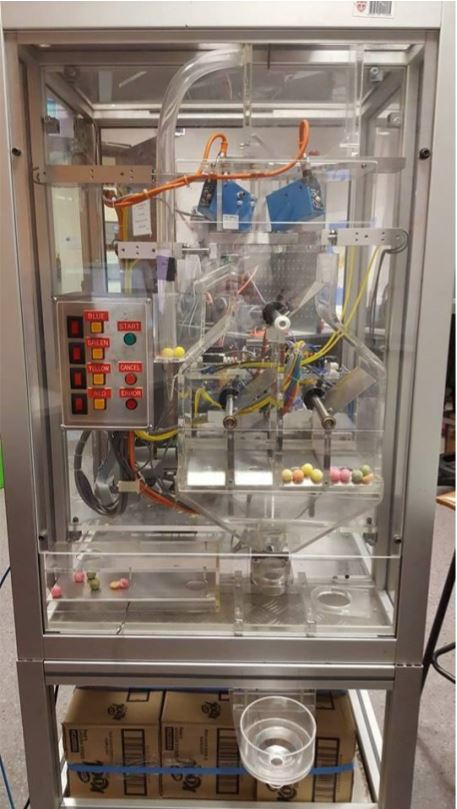
\includegraphics[scale = 0.5]{lollyMachine.JPG}
        \caption{The lolly machine~\cite{thesisJodie}.}
        \label{fig:lollyMachine}
    \end{figure}

    \newpage

\chapter{Background}
    \label{chap:background}
    

% should i preface the reader with the reason for the background?
% what is the reason for the background?
The lolly machine is comprised of many different components from pneumatic actuators to industrial communication protocols - most of which do not come under the banner of common knowledge. The background section aims to preface the reader with all necessary information required to understand all components, hence allowing the reader to comprehend the work that has been completed. 

\section{Pneumatics}
    Pneumatics is a category of mechanical engineering  where air flow is converted into mechanical energy\cite{parr2011hydraulics}. The mechanical energy is then used to do work. A typical application of pneumatics is to move an actuator from one position to another, i.e. from open to closed. Pneumatics are common within the food processing industry as a malfunction within the system will not spoil the product.
    All mechanical movement within the lolly machine is driven by pneumatic actuators.
    
\section{Linear Actuators}
    Linear actuators, as the name suggests, provides linear movement to push and/or pull objects within a given process. The linear actuators on the lolly machine are powered by pneumatics. The main components of a linear actuator are as follows:
    
    \begin{description} 
        \item\textbf{Rod:} connects the actuator to the outside environment.
        \item\textbf{Piston:} facilitates movement to the rod through applied pressure to either side.
        \item\textbf{Barrel:} houses the piston.
        \item\textbf{Extend Port:} when air enters, the rod will extend outwards.
        \item\textbf{Retract Port:} When air enters, the rod will retract inwards.
    \end{description}
    
    The fundamental concept is that the differential pressure between either side of the piston will cause it to move\cite{parr2011hydraulics}. The direction of movement is dependent on the flow of air through the extend and retract ports.
    
    
    There are eight linear actuators installed on the lolly machine. Three are used within the sorting process while five are required for dispensing. Figure \ref{fig:rejectAct} shows the linear actuator responsible for dropping lollies into the colour sensing shoot.

    \begin{figure}[H] 
        \centering
        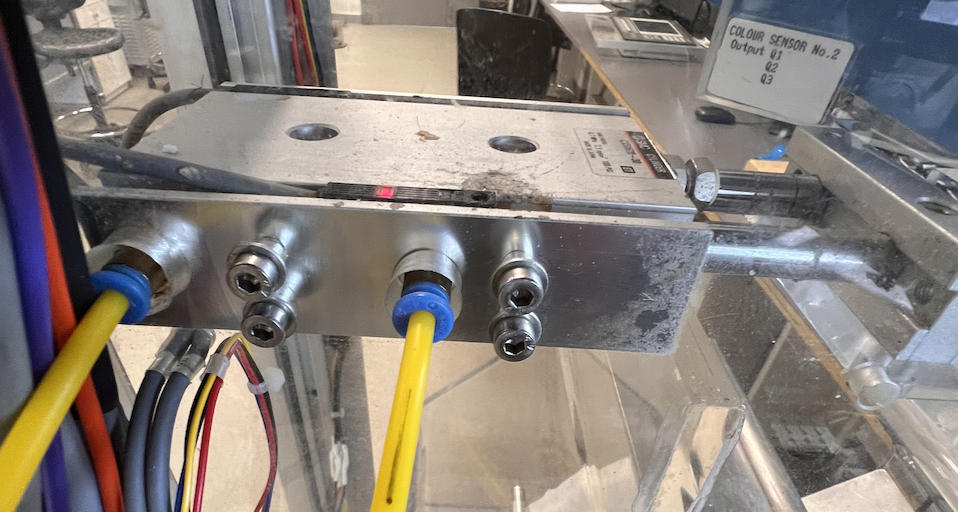
\includegraphics[width = 0.5\textwidth]{2_images/rejectAct.png}
        \caption{Lolly machine reject actuator.}
        \label{fig:rejectAct}
    \end{figure}        
    
\section{Rotary Actuators}
    Rotary actuators provide rotational movement to objects through a central shaft\cite{parr2011hydraulics}. Rotation can be restricted or unrestricted. A rack and pinion or vanes facilitate the turning action within the actuator\cite{parr2011hydraulics}. Rotary actuators within the lolly machine are driven by a single vane and restricted to 90$^{\circ}$\cite{smcRot}. There are three rotary actuators installed on the lolly machine.

\section{Pneumatic Control Valves}
    The pneumatic control valves on the lolly machine, manage air flow to pneumatically driven actuators. Pneumatic control valves are defined by the number of ports, positions, and their control action\cite{parr2011hydraulics}. Figure \ref{fig:controlValves} compares two different types of valves - (a) shows a four-port two-position valve (4/2) while (b) shows a four-port, 3-position valve(4/2). Figure \ref{fig:controlValveConfig} shows a possible internal configuration for the 4/3 valve. It is important to note that the above mentioned figures do not represent typical pneumatic valve symbols and are included to illustrate the differences between various types of control valve configurations.
    
    \begin{figure}[H]
    \centering
    \begin{minipage}{0.45\textwidth}
        \centering
        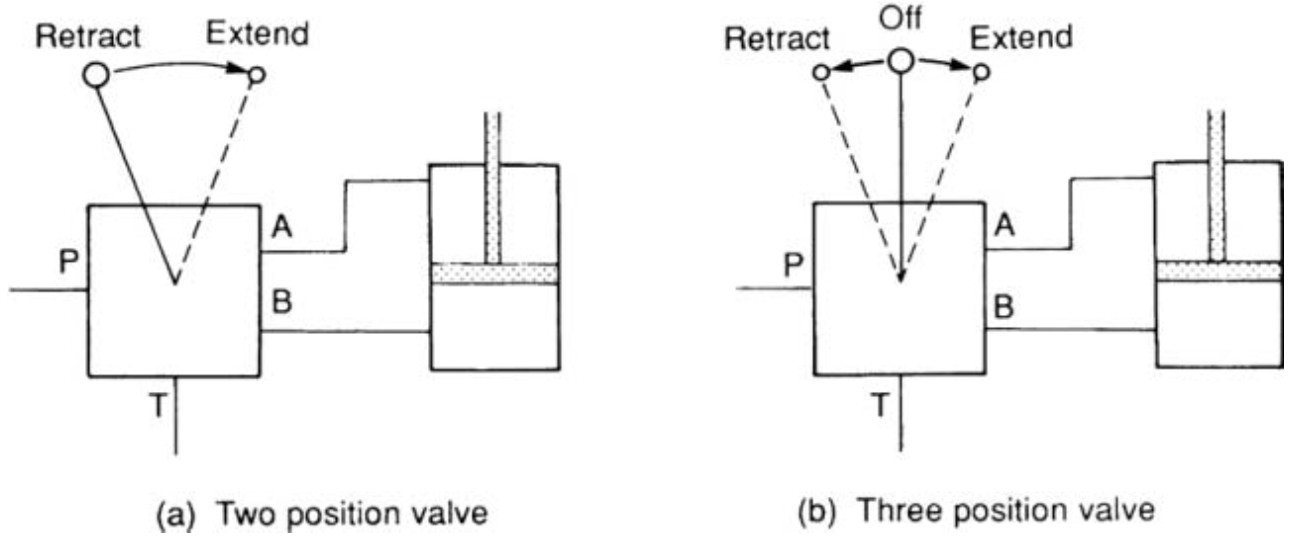
\includegraphics[width = 1\textwidth]{2_images/controlValves.png}
        \caption{Comparison between control valves~\cite{parr2011hydraulics}.}
        \label{fig:controlValves}
    \end{minipage}\hfill
    \begin{minipage}{0.5\textwidth}
        \centering
        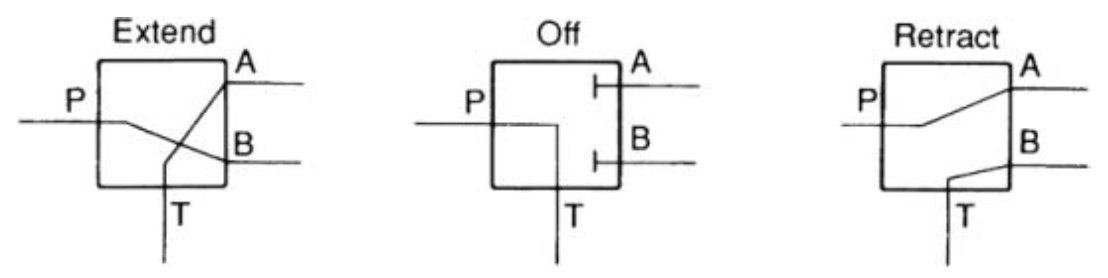
\includegraphics[width = 1\textwidth]{2_images/controlValveConfig.png}
        \caption{4/3 control valve switching configuration~\cite{parr2011hydraulics}.}
        \label{fig:controlValveConfig}
    \end{minipage}\hfill            
    \end{figure}      

    All actuators on the lolly machine are driven by 5/2 control valves, this means that each valve has two positions and 5 ports. Figure \ref{fig:5_2Valve} shows a 5/2 pneumatic valve symbol. Valve positions are shown by two square boxes (coloured red and green to clearly illustrate the different positions) each containing two arrows and a T. The arrows show the air flow direction between ports while the T represents a plug. The zigzag on the right hand side of the symbol illustrates a spring, indicating the the control valve is spring return. The rectangle with the diagonal line through the middle shows that a solenoid drives the control action. Figure \ref{fig:cylinderAB} shows the two possible positions of the cylinder.

    \begin{figure}[H]
    \centering
    \begin{minipage}{0.45\textwidth}
        \centering
        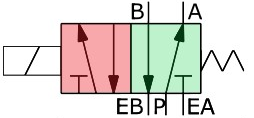
\includegraphics[scale = 0.5]{2_images/5_2Valve.png}
        \caption{A 5/2 pneumatic control valve \cite{5_2Valves}.}
        \label{fig:5_2Valve}
    \end{minipage}\hfill
    \begin{minipage}{0.5\textwidth}
        \centering
        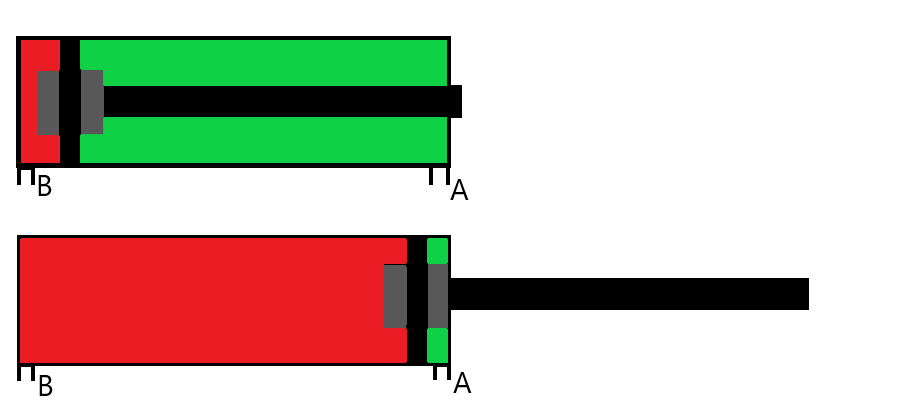
\includegraphics[width = 0.8\textwidth]{2_images/cylinderAB.png}
        \caption{Different cylinder positions. \\Position 1(Top) = Retracted. \\Position 2(Bottom) = Extended}
        \label{fig:cylinderAB}
    \end{minipage}\hfill            
    \end{figure}          
   
   The below position descriptions are in reference to Figure \ref{fig:5_2Valve}.
    \begin{description}
        \item\textbf{Position 1 - Green:}
        While the valve is in position 1 the pressure (P) port is connected to the (A) port and (B) port is connected to the exhaust line (EB).
        \item\textbf{Position 2 - Red:}
        While the valve is in position 2 the pressure (P) port is connected to the (B) side and (A) port is connected the exhaust line (EA). 
    \end{description}
    
    The control action is what triggers the pneumatic control valve and can vary depending on the application, typical control actions include\cite{parr2011hydraulics}:
    \begin{itemize}
        \item Push Button
        \item Spring
        \item Lever
        \item Roller Limit Switch
        \item Pressure Line
        \item Solenoid
    \end{itemize}
    
    All control valves on the lolly machine are are triggered via solenoid driven pilot valves.

\section{I/O}
    
    \acrfull{io}, as the name suggests, are the inputs and outputs of a control system. Inputs are often referred to as sensors as they are devices that translate a real world signal into something that the \acrshort{cpu} can make sense of - this typically consists of some sort of electrical signal (Voltage or Current). Outputs, on the other hand, are often referred to as "final control elements" or "actuators". Output devices are how the control system is able to interact with the outside world.\\
    There are four main types of \acrshort{io}:

    \begin{description}
    \item\textbf{Digital Inputs} - Binary input signals (On or Off).
    \item\textbf{Digital Outputs} - Binary output signals (On of Off).
    \item\textbf{Analog Inputs} - Variable electrical (voltage or current) inputs signals.
    \item\textbf{Analog Outputs} - Variable electrical (voltage or current) output signals.
    \end{description}
    
    The lolly machine \acrshort{io} is comprised of digital inputs and outputs. This section will provide a brief overview to all different types of digital \acrshort{io} that can be found on the lolly machine

\subsection{Inputs}
    \subsubsection{Limit Switches}
        Magnetically activated limit switches manufactured by \acrshort{smc} provide actuator position feedback. There are two limit switches installed on each actuator, one that activates when the actuator is fully extended and the other when it is fully retracted. The limit switches are installed within a track on the actuator and held in place by a small grub screw - this can be seen in Figure \ref{fig:rejectAct}.
        The limit switches have an internal solid state circuit that is activated when the piston is adjacent. The piston is made from a magnetic ferrous material which is what allows the switch to activate. 
        Figure \ref{fig:autSwShm} shows the internal electrical schematic of the \acrshort{smc} limit switches.
        
        \begin{figure}[H]
            \centering
            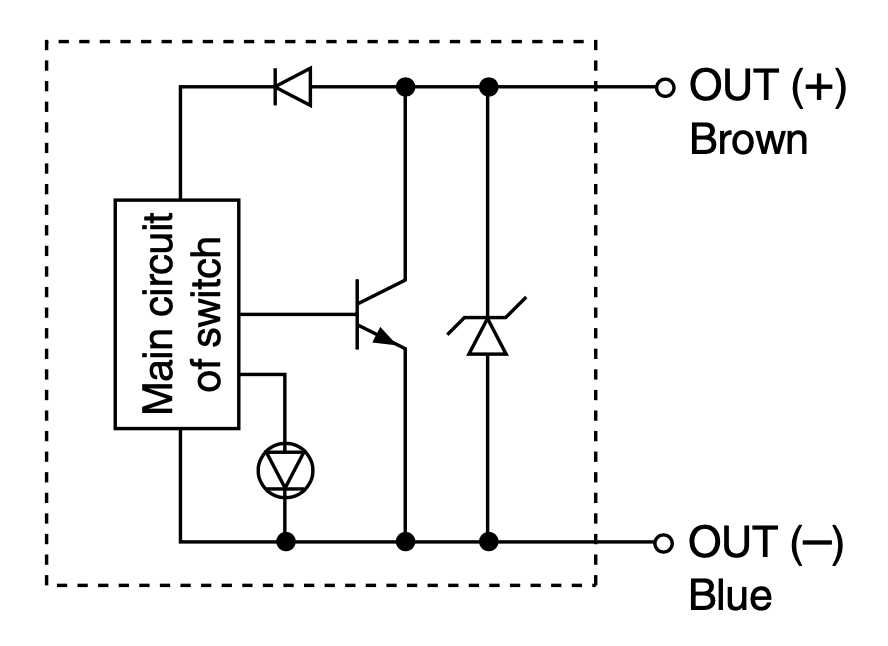
\includegraphics[scale = 0.4]{2_images/autSwShm.png}
            \caption{Internal electrical schematic of an \acrshort{smc} limit switch~\cite{smcRot}.}
            \label{fig:autSwShm}
        \end{figure}

    \subsubsection{Proximity Sensors}
        Two proximity sensors are installed on the lolly machine. The sensors determine whether or not a lolly is in situ. The proximity sensors installed on the lolly machine are capacitive; this allows the sensors to detect ferrous and non-ferrous materials. Figure \ref{fig:proxSens} illustrates the general function of a proximity sensors. In the case of the lolly machine, the proximity sensors are \acrshort{nc} which means that the output is on when the target is detected and off while the target is not.
    \begin{figure}[H]
    \begin{minipage}{0.35\textwidth}
        \centering
            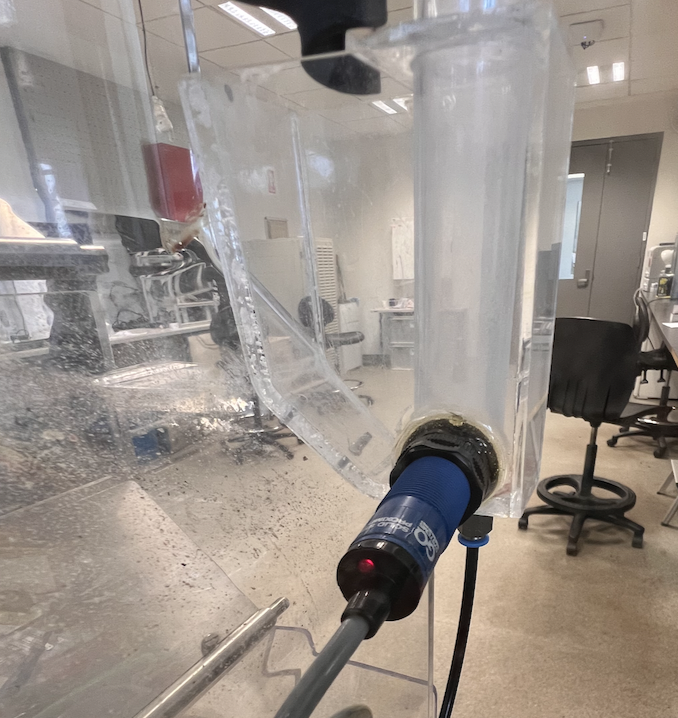
\includegraphics[scale = 0.4]{2_images/rejectProx.png}
            \caption{Lolly machine proximity sensor used to detect when a lolly is in the reject bucket.}
            \label{fig:rejectProx}
    \end{minipage}\hfill
    \begin{minipage}{0.35\textwidth}
        \centering
        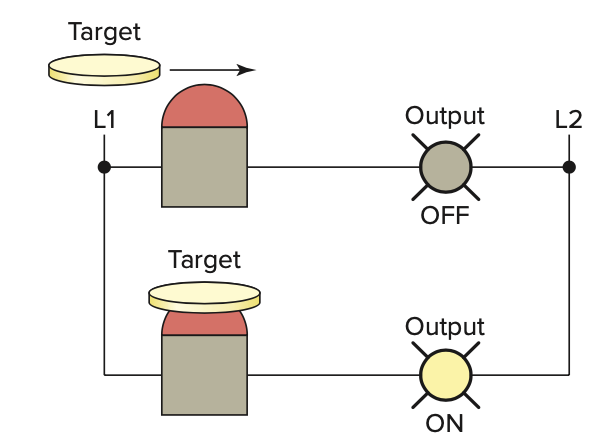
\includegraphics[width = 0.9\textwidth]{2_images/proxSens.png}
        \caption{Typical function of a proximity sensor \cite{petruzella2017programmable}.}
        \label{fig:proxSens}
    \end{minipage}\hfill 
    \end{figure}
    
    \subsubsection{Colour Sensors}
        The colour sensors onboard the lolly machine emit Red, Green and Blue light onto each passing lolly, the radiation reflected off the lollies is detected and compared to previously stored/ learned coordinates within the sensor \cite{sickColourSenors}. If the detected radiation of the lolly is within a certain tolerance of the learned coordinates then an output from the sensor is set to true, indicating that a desired colour has been detected. There are two "SICK" colour sensors on-board the lolly machine - one that can detect three different colours while the other, only one.
        %Although the colour sensors used on the lolly machine can’t actually detect the complete range of colours which can be seen by us, the two colours sensors (3 digital signals from one sensor, and 1 digital signal from the second), are able to be “trained/calibrated” to provide an indication of a number of different colour matches.
        Figure \ref{fig:cs1} shows the electrical connections of one of the colour sensors while Figure \ref{fig:colSens} shows a picture of the colour sensors installed on the machine.

        \begin{figure}[H]
            \centering
            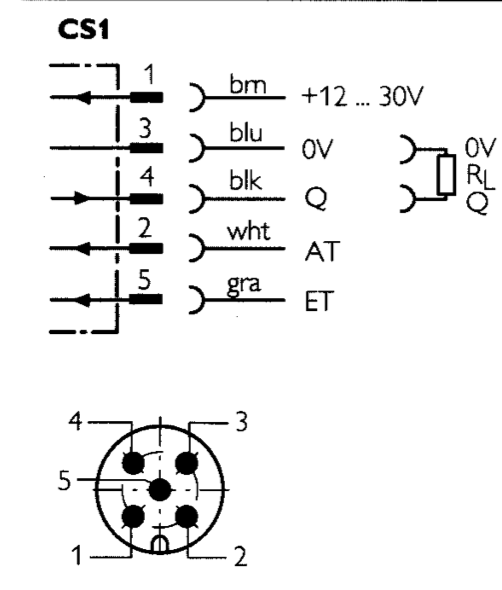
\includegraphics[scale = 0.4]{2_images/cs1.png}
            \caption{Electrical connections for a single output colour sensor \cite{sickCs}.}
            \label{fig:cs1}
        \end{figure}     
        
        \begin{figure}[H]
            \centering
            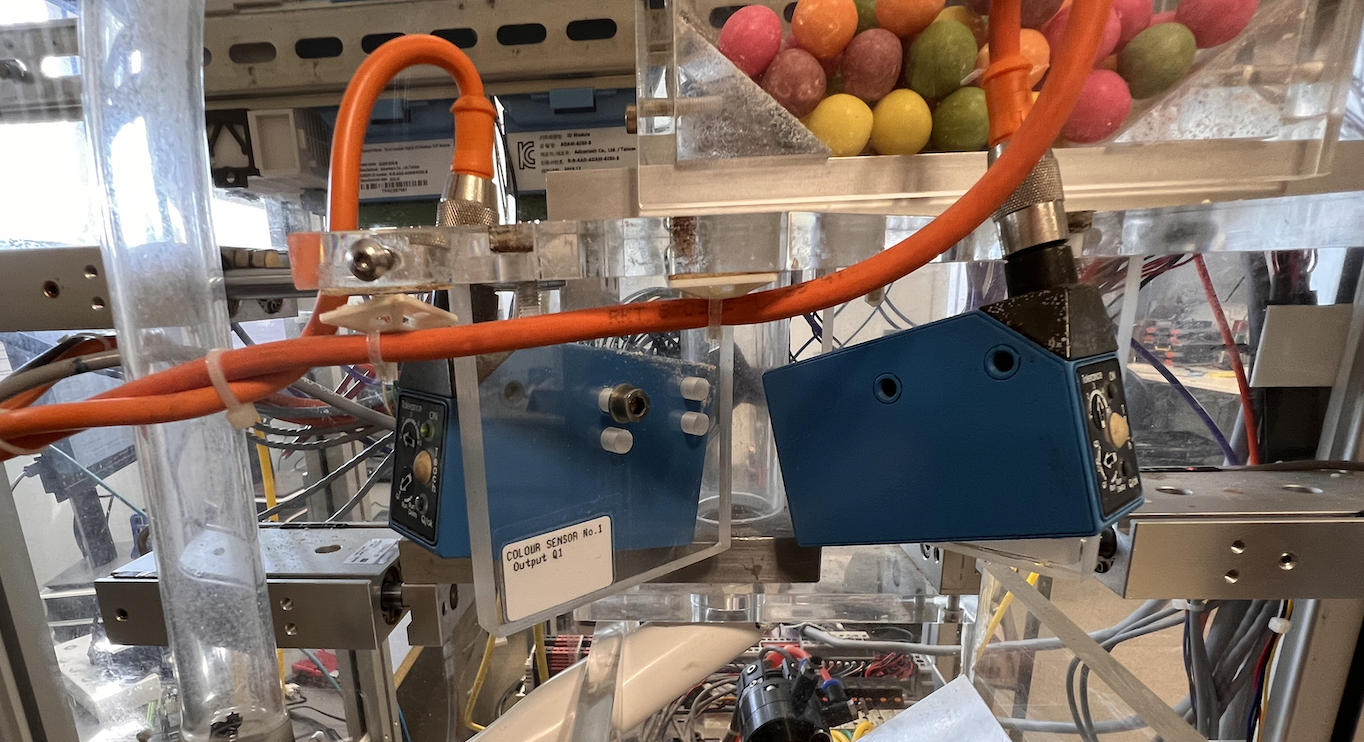
\includegraphics[scale = 0.4]{2_images/colSens.png}
            \caption{The two lolly machine colour sensors.}
            \label{fig:colSens}
        \end{figure}       

    \subsubsection{Buttons}
    Physical push buttons provide an interface between the operator and the machine where different buttons are linked to different machine functions. For example, an \acrfull{estop}, when pressed, will halt the operation of the machine and put it into error mode. While in error mode, the machine will cease to operate until it has been an given instruction by the user that it is safe to do so. The \acrshort{estop} is a \acrshort{nc} contact while the rest of the buttons on the machine are \acrshort{no}.
    %Find a figure of a NO button - can probably find in the PLC book
    
\subsection{Outputs}
    \subsection{Solenoids - Pneumatic Valve}
    All pneumatic actuators on the lolly machine are activated by pneumatic control valves. The control valves are activated by an internal solenoid driven pilot valve.  The output device, from the perspective of the \acrshort{plc}, is the solenoid. The fundamental components of a solenoid are a wire coil and ferrous core. The ferrous core is located within the coil. When a \acrshort{dc} voltage is applied to the coil it behaves like a magnet, this is called an electromagnet. When the solenoid is switched, the ferrous core moves from one end of the solenoid housing to the other. The core is connected to the pilot valve which provides the necessary mechanical action to change the valve position, which in turn, moves the actuator. 
    
        \begin{figure}[H]
            \centering
            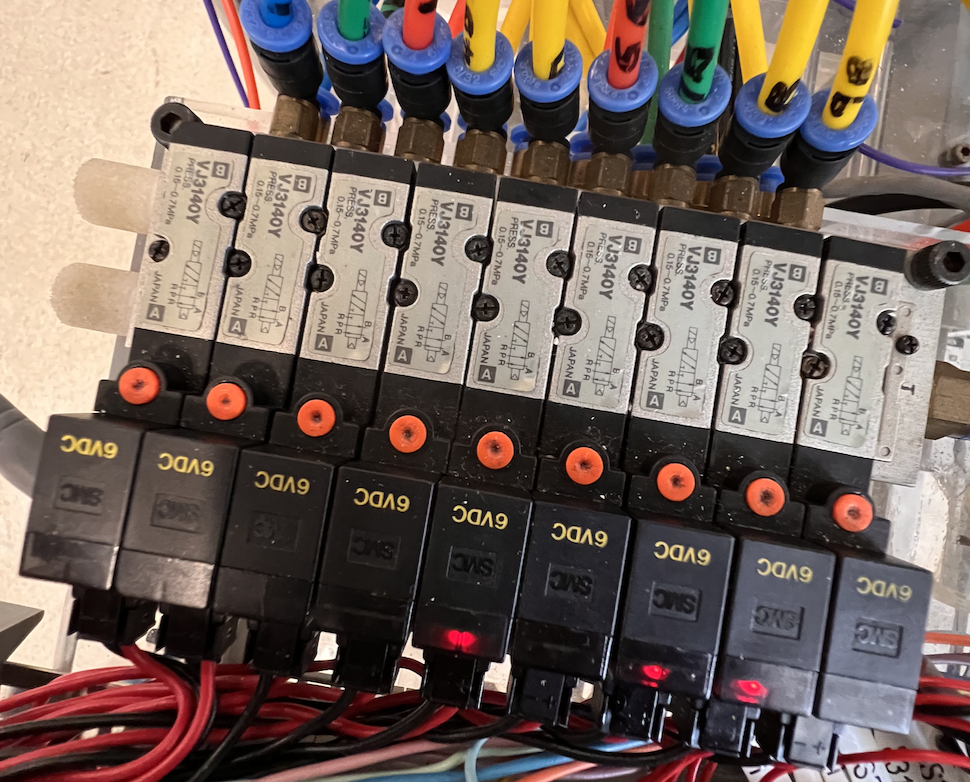
\includegraphics[scale = 0.5]{2_images/controlValvesPic.png}
            \caption{Solenoid pneumatic control valves mounted on manifold.}
            \label{fig:controlValvesPic}
        \end{figure} 
    \newpage
    \subsubsection{\acrshort{led} Indicators}
        A number of \acrshort{led} based lights are used on the lolly machine. The \acrshort{led}s are linked to specific machine states and will either be on, off  or flashing. \acrshort{led}s are robust, lasting much longer than previously used incandescent lights. As most \acrshort{led}s require only a couple of volts, all have internal series resistors which allows all \acrshort{led}s on the lolly machine to be directly controlled and switched by the \acrshort{plc}.
        
        \begin{figure}[H]
            \centering
            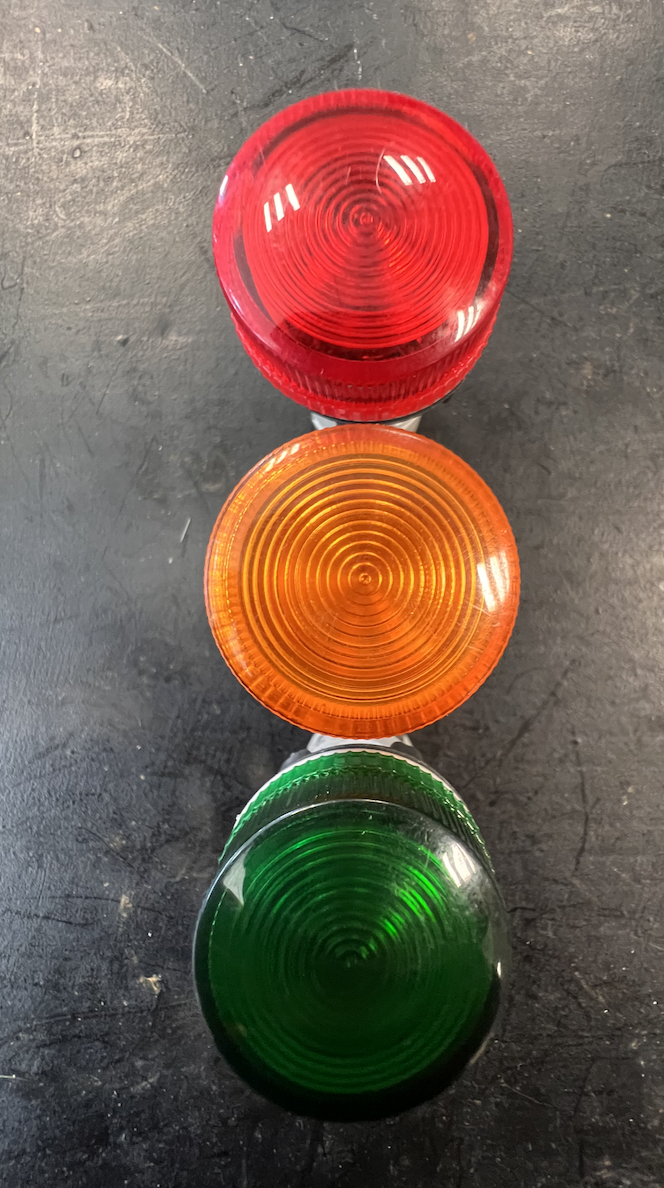
\includegraphics[scale = 0.3]{2_images/leds.png}
            \caption{Lolly machine \acrshort{led}s}
            \label{fig:leds}
        \end{figure} 
        
%There are two main streams of process control - continuous and sequential\cite{dunn2006introduction}. Continuous control involves the constant monitoring and manipulation of dynamic systems while while sequential control is event based. Given the nature of the lolly machine, sequential control is the obvious choice for controlling the system \cite{dunn2006introduction}.

The lolly machine is, in essence, an automatic machine. This section investigates various components that facilitate the automation aspects of the project.

\section{State Machine Design}
    State machine design, sometimes refereed to as sequential machine design, is a systematic method of programming which is commonly used to structure and machine code. Different variations of state machine design exist within industry and sometimes they can be difficult to identify, making the code look unnecessarily complicated and confusing to read. State machine design is comprised of different states with transitions between states. Actions within each state define how the machine will behave in said state while transitions between states are the conditions than need to exist to allow the machine to transition from one state to another. Figure \ref{fig:stateMachineEx} shows the general concept of state machine design. State machine design can be written in arguably any language. Some languages, like GRAPH by Siemens, are based on the concept of state machine design as evident by the look and feel of the language. 

    \HD{If you get time - find a reference that backs up what you have said here about state machine design}

        \begin{figure}[H]
        \centering
        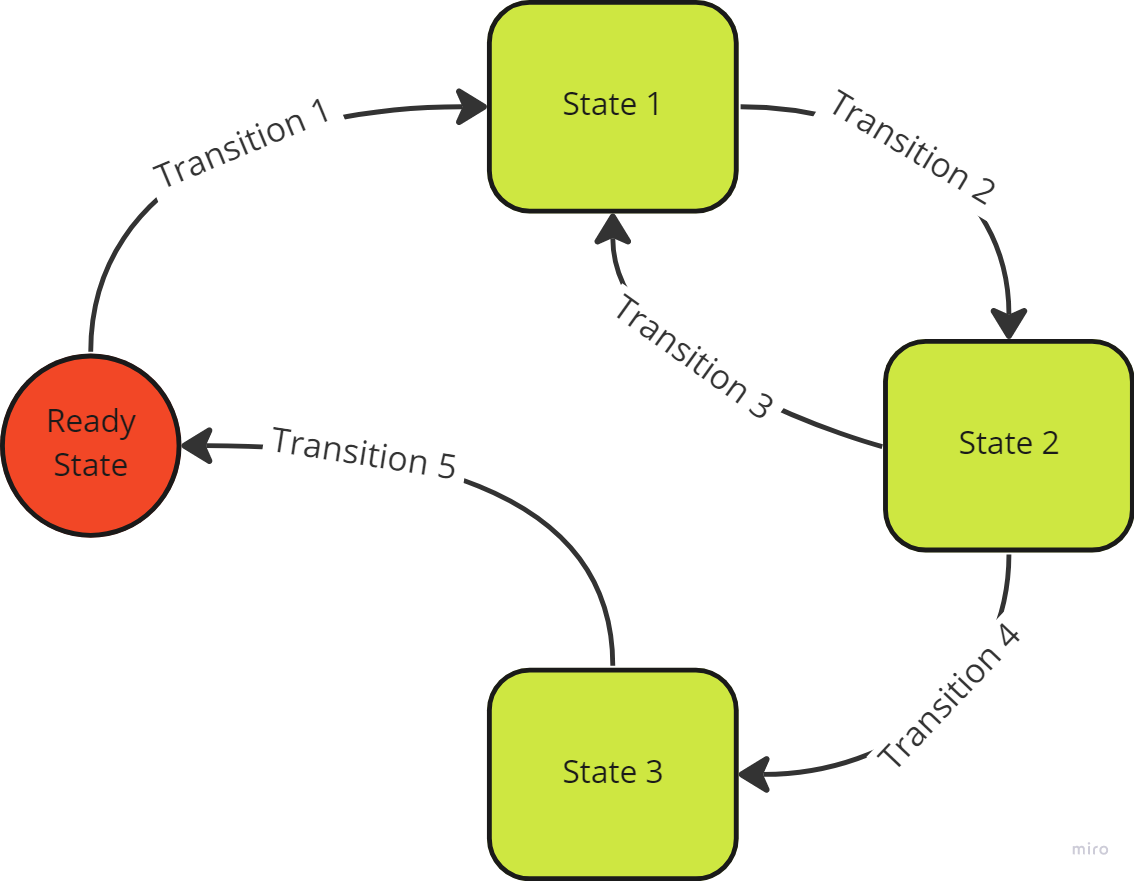
\includegraphics[width = 0.5\textwidth]{2_images/stateMachineEx}
        \caption{The general concept behind state machine design.}
        \label{fig:stateMachineEx}
    \end{figure}

\section{Programmable Logic Controller (PLC)}


    A \acrfull{plc} is an industrial controller/ computer that can be programmed to perform specific \acrshort{rt} tasks and can utilised for varying applications\cite{petruzella2017programmable}. A \acrshort{plc} performs these tasks through solving logic based operations\cite{petruzella2017programmable}.  E.g., if a water tank is filled to a level which is deemed "to high" turn off the water supply to the tank. A \acrshort{plc} interacts with the outside world through the use of either onboard or remote \acrshort{io}.
    
    Prior to the existence of \acrshort{plc}s, sequential based control was performed through relay\footnote{Relays are an electrical component comprised of a solenoid and contacts(\acrshort{no} and/or \acrshort{nc}), when the solenoid is energised the contacts change state.}-logic. Relay logic required multiple relays to be wired in a certain configuration allowing for the control of the system. Figure \ref{fig:relayLogic} shows an example of a relay-logic based control system\cite{petruzella2017programmable}. 
    \acrshort{plc}s provided a much cleaner, organised and easier to troubleshoot method of control as seen in Figure \ref{fig:plcLogic}.    
    
    \begin{figure}[H]
    \centering
    \begin{minipage}{0.35\textwidth}
        \centering
        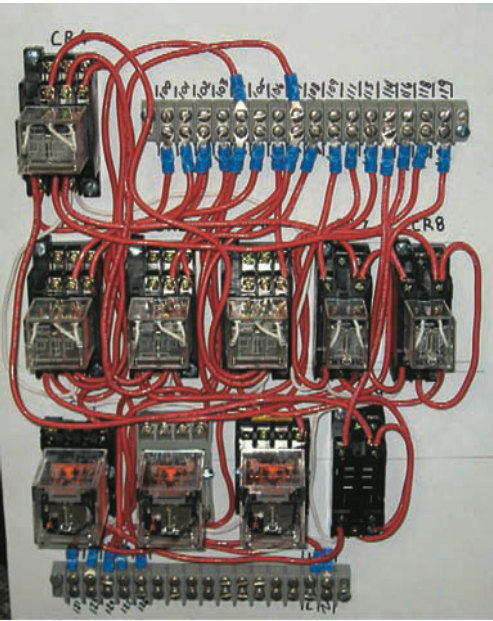
\includegraphics[width = 0.9\textwidth]{2_images/relayLogic.png}
        \caption{Relay logic based control system.~\cite{petruzella2017programmable}}
        \label{fig:relayLogic}
    \end{minipage}\hfill
    \begin{minipage}{0.35\textwidth}
        \centering
        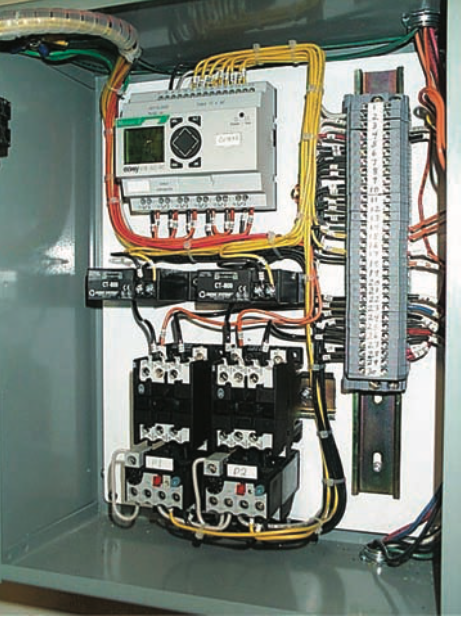
\includegraphics[width = 0.9\textwidth]{2_images/plcLogic.png}
        \caption{\acrshort{plc} based control system.~\cite{petruzella2017programmable}}
        \label{fig:plcLogic}
    \end{minipage}\hfill            
    \end{figure}   
    
    Originally, \acrshort{plc}s where exclusively programmed in a language called \acrfull{ld}\cite{petruzella2017programmable}. Ladder logic is a visual programming language based on electrical control schematics and was designed to be used by the same people who were building the relay logic based control systems ,electricians\cite{petruzella2017programmable}. In more recent times \acrshort{plc}s have become more sophisticated and can be programmed in a variety of languages including \acrfull{st} which is a text based language\cite{petruzella2017programmable}. 
    
    A \acrshort{plc}'s main components are a power supply, \acrlong{cpu}, and \acrshort{io} modules. \acrshort{io} modules can be located locally or remotely. Local \acrshort{io} is physically connected to the \acrshort{plc} while remote \acrshort{io} is connected to the \acrshort{plc} via a communication line, this is illustrated in Figure \ref{fig:localRemoteIo}.
       
    \begin{figure}[H]
        \centering
        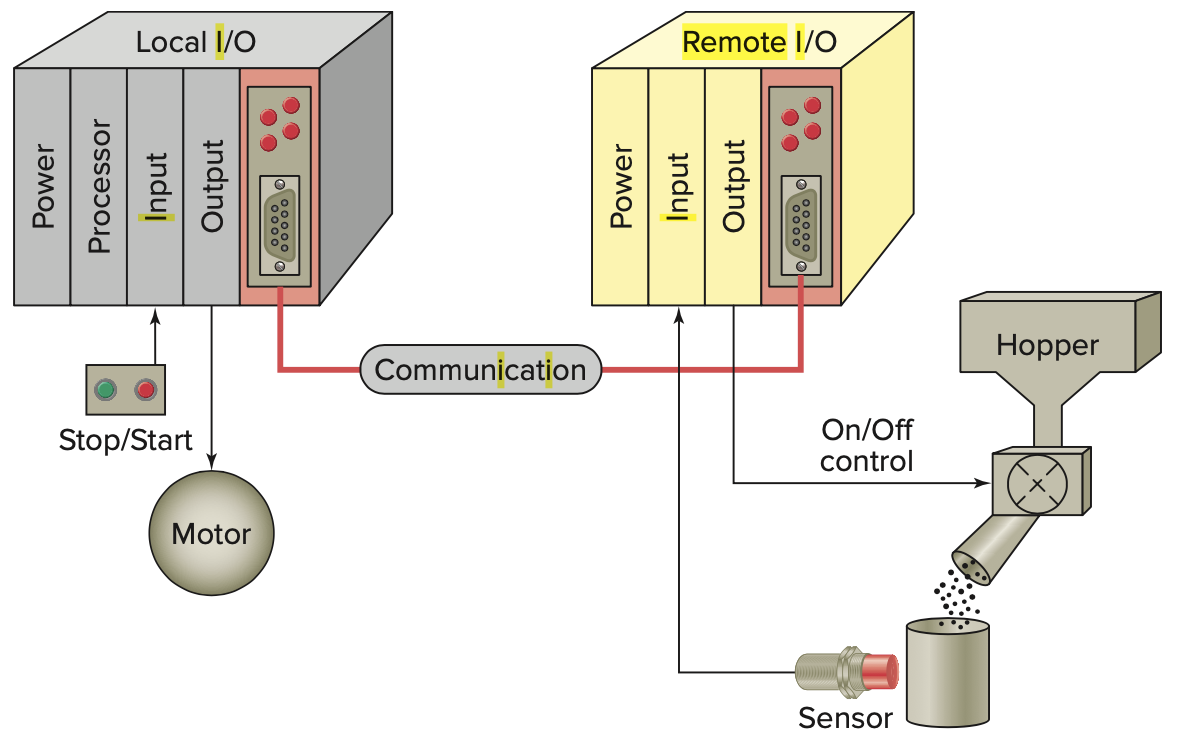
\includegraphics[width = 0.5\textwidth]{2_images/localRemoteIo.png}
        \caption{Local and remote \acrshort{io}}
        \label{fig:localRemoteIo}
    \end{figure}
 
\section{Human Machine Interface (HMI)}
    A \acrfull{hmi}, as the name suggests, is the interface between the machine and the human/ operator. A \acrshort{hmi} is a screen that shows the machine state through graphics. An operator enters commands through the touch screen or a keyboard and mouse. \acrshort{hmi}s are programmable and can be used to control and monitor almost any machine\cite{petruzella2017programmable}. Typically, there is one \acrshort{hmi} per machine/ operator. It is not uncommon to have multiple \acrshort{hmi}s within a single factory. Figure \ref{fig:typHmi} shows an example of what a \acrshort{hmi} screen for a basic motor controller might look like.

    \begin{figure}[H]
        \centering
        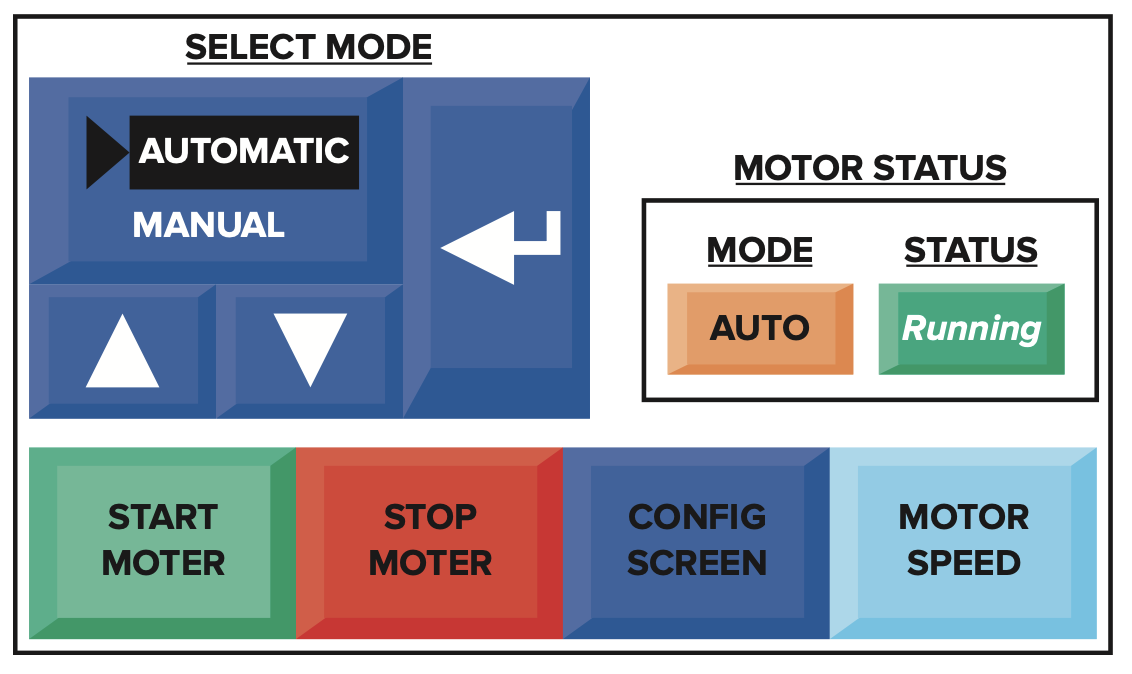
\includegraphics[width = 0.5\textwidth]{2_images/typicalHmi.png}
        \caption{A typical \acrshort{hmi} motor controller screen\cite{petruzella2017programmable}}
        \label{fig:typHmi}
    \end{figure}    
    
\section{Engineering Workstation}
    An engineering workstation is a \acrshort{pc} that has been set up for a engineer. The engineering workstation is connected to the \acrshort{ot} network and setup with all relevant software specific to the controlled process. In the case of the lolly machine the engineering workstation is a desktop computer that has all of the necessary  software to connect, configure and program all system hardware. 
\section{Microcontrollers}
    To understand what a microcontroller is, a few definitions must be made \cite{crisp2003introduction}.
    
\begin{description}
    \item{\textbf{Integrated Circuits:}} - An electronic circuit that is printed onto solid block. The circuit contains semi-conductor components. Integrated circuits are often referred to as chips.
    \item{\textbf{Microprocessor:}} - A microprocessor is part of a system, it is the central processing unit and is useless without surrounding circuitry and applied voltages.
    \item{\textbf{Microprocessor-based System:}} A microprocessor-based System is any system that is controlled by a microprocessor. 
\end{description}    
    
    A \textbf{microcontroller} is a microprocessor-based embedded system built into an integrated circuit and is usually capable of controlling its own \acrshort{io} \cite{crisp2003introduction}.
    
    Microcontrollers are capable of performing an almost infinite list of tasks, e.g., controlling a wrist watch, monitoring and controlling a home irrigation system or controlling a robot. Some micorcontrollers, like the ones in a wrist watch or calculator,  can not be easily programmed after they leave the factory while other can.
    
    Similar to a \acrshort{plc}, micorcontrollers have onboard \acrshort{io} with the caveat being the hyper sensitivity to voltages above the standard operating voltage of the microcontroller which is typically 3.3 volts. Two micorcontrollers are used on the lolly machine - these are a Raspberry Pi and an Arduino.  
  
    \begin{figure}[H]
    \centering
    \begin{minipage}{0.4\textwidth}
        \centering
        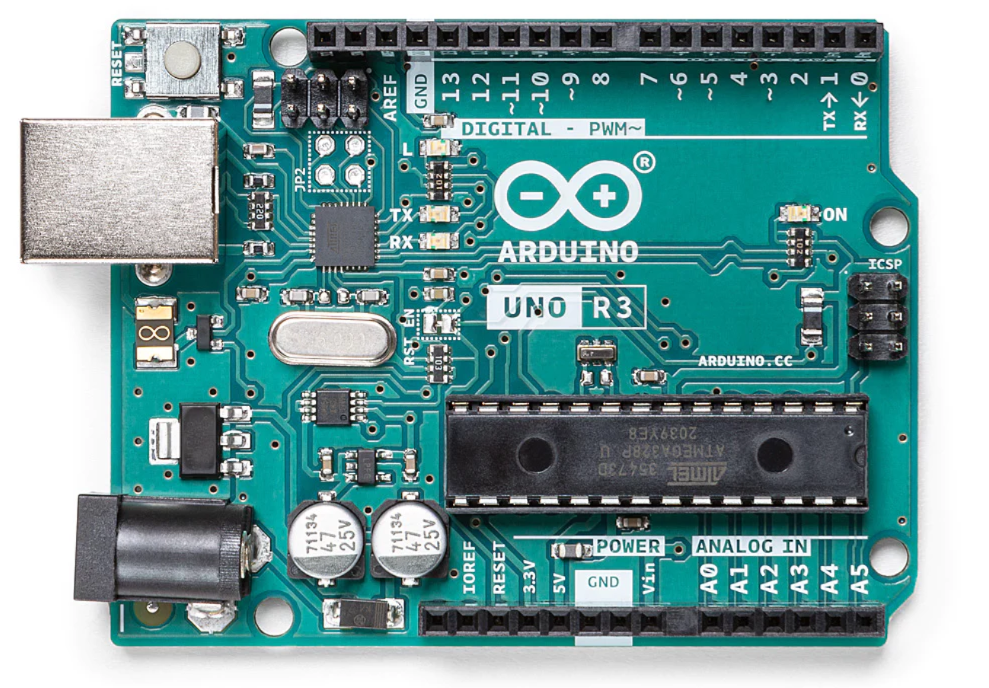
\includegraphics[width = 0.8\textwidth]{2_images/arduino.png}
        \caption{An Arduino~\cite{arduinoWeb}}
        \label{fig:arduino}
    \end{minipage}\hfill
    \begin{minipage}{0.4\textwidth}
        \centering
        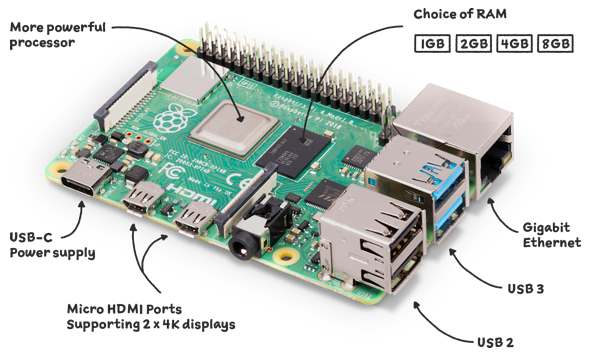
\includegraphics[width = 0.9\textwidth]{2_images/RaspPi.png}
        \caption{A Raspberry Pi~\cite{raspPiWeb}}
        \label{fig:raspPi}
    \end{minipage}\hfill            
    \end{figure}     

\subsection{Data Types}
    Data types represent different numerical formats within a process control system. Most variables within the lolly machine are Boolean (bit). The below list defines the basic data types used within a process control system. 
    
    \begin{table}
    \centering
    \caption{Data types of a typical control system.}
        \begin{tabular}{ |p{3cm}|p{2cm}|p{3cm}|  }
                \hline
                \multicolumn{3}{|c|}{\textbf{Data Types}} \\
                \hline
                \textbf{Type}& \textbf{Bits}& \textbf{Example} \\
                \hline
                Bit & 1 & True/False or 1/0 \\
                Byte & 8 & 16\#8 or 00001000 \\
                Word & 16 & 16\#F8 \\
                Double Word & 32 & 16\#FF00 \\
                Integer & 16 & '123' \\
                Float or Real & 32 & '123.45'\\
                \hline
        \end{tabular}
        \label{table:dataTypes}   
        
    \end{table}
    

        \begin{figure}[H]
            \centering
            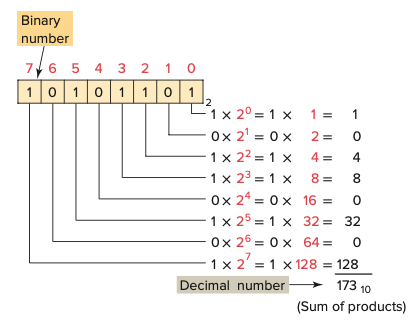
\includegraphics[width = 0.4\textwidth]{2_images/int.png}
            \caption{An 8 bit integer \cite{petruzella2017programmable}.}
            \label{fig:int}
        \end{figure}         

\section{Communication}

\subsection{Serial}
    Serial communication is a method of data transfer between devices where data is transmitted and received one "bit" at a time \cite{frenzel2015handbook}. Communication is typically facilitated through copper wires where data is represented by electrical signals. Serial communication standards define the specifics as to exactly how the data is transferred and interpreted. Below are some basic descriptions of a few common terms used within serial communication.
    
    \begin{description}
    
    \item[Baud Rate] The baud rate refers to the speed of data transfer. More specifically it refers to how many bits are able to be transmitted and received per second. 
    
    \item[Communication Mode] There are three different types of communication modes: Simplex, Half Duplex and Full Duplex. For the sake of simplicity, the following explanations are in reference to a peer-to-peer system comprising of only two devices, lets call them Device-A and Device-B. Simplex means that communication is one way - Device-A is capable of transmitting data while device-B is capable of only receiving data.
    
    \item[Asynchronous/ Synchronous] Data transmission can be achieved through either synchronous or asynchronous methods of communication. \HD{Explain the differences and don't forget to reference.}
    
    \end{description}
    
    The lolly machine utilises three flavours of serial communication, these are as follows.
    
    \subsubsection{RS-232}
    RS-232 has been around for a long time and is one of the older methods of serial communication. Although there are many superior methods of communication in this modern era, RS-232 is still common among industry. 
    RS-232 is supported by the Click \acrshort{plc}. During normal operation, the \acrshort{plc} communicates to all system peripherals through an Ethernet protocol and does not require RS-232. Unfortunately, the \acrshort{plc} factory settings do not include a static \acrshort{ip}\footnote{An \acrshort{ip} address is a unique address required for the type of communication network (router-less Ethernet) that that has been implemented on the lolly machine} address.  RS-232 is used exclusively for setting the \acrshort{ip} address of the \acrshort{plc}. Figure \ref{fig:rs232Trans} shows a typical RS-232 data transmission. 

    \begin{figure}[H]
        \centering
        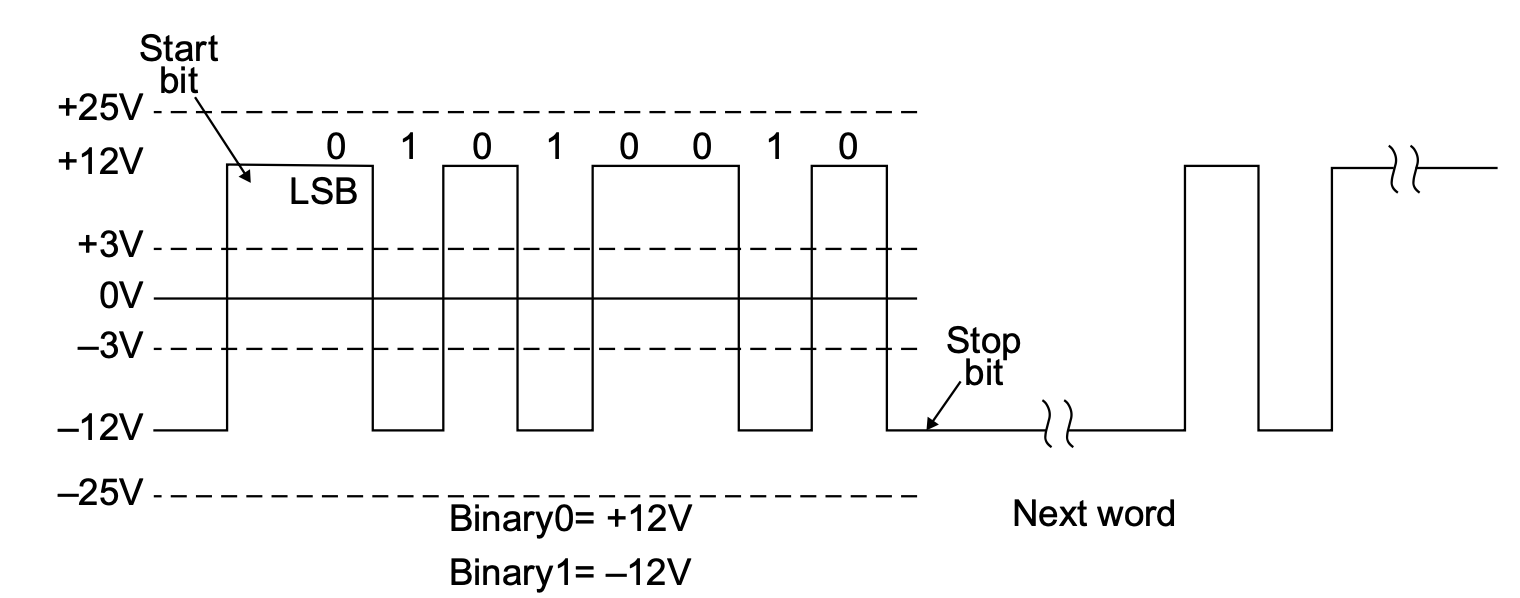
\includegraphics[width = 0.7\textwidth]{2_images/rs232Trans.png}
        \caption{A RS-232 data transmission~\cite{frenzel2015handbook}.}
        \label{fig:rs232Trans}
    \end{figure} 
    \newpage    
    
    \subsubsection{RS-485}
    The RS-485 serial protocol is used for communication between the Arduino and the \acrshort{plc}.
    
    \subsubsection{SPI}
    The SPI protocol is used to link the Arduino to the \acrshort{rgb} \acrshort{led}s.
    
    % could also include spi and i2c but we will see. . . 

 
     
\subsection{Ethernet}
    Ethernet, also known as IEEE 802.3, is a commonly used communication standard that governs the Physical and Data-Link Link layers (in relation to the \acrshort{osi}\footnote{The \acrshort{osi} model provides a framework that describes how applications can communicate over a wired \acrshort{lan}\cite{scott2021networking}.} model shown in Figure \ref{fig:osi}) of a wired \acrshort{lan}\cite{scott2021networking}. A wired \acrfull{lan} is a group of network devices that are connected on a local Ethernet network.  
    
        \begin{figure}[H]
            \centering
            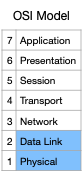
\includegraphics[width = 0.1\textwidth]{2_images/osi.png}
            \caption{The \acrshort{osi} model\cite{scott2021networking}.}
            \label{fig:osi}
        \end{figure} 
    
    An Ethernet network is established through physical cabling. Cabling can be coaxial, twisted copper pairs of fibre optic \cite{scott2021networking}.
    
    All devices on the lolly machine support Ethernet, subsequently all devices are on the same \acrshort{lan}.
    
    Each Ethernet device has a unique address which is called an \acrshort{ip} address. An \acrshort{ip} address is a four-octet, eight-bit address\cite{scott2021networking}.  
    
    \begin{figure}[H]
        \centering
        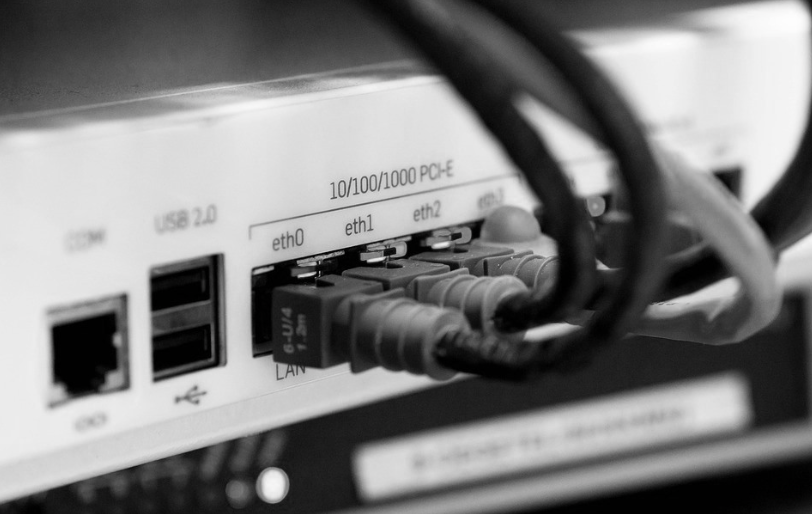
\includegraphics[width = 0.6\textwidth]{2_images/ethernetCables.png}
        \caption{Ethernet cables plugged into a network switch\cite{scott2021networking}.}
        \label{fig:ethenetCables}
    \end{figure} 

    There are two main types of Ethernet devices - Client device and Server device. To best explain the relationship between Client and Server devices, the following analogy can be used. In a restaurant, the customer requests food from the waiter. The waiter listens to the customers request and proceeds to deliver the food back to the customer. If you haven't already guessed, the customer is the Client, the waiter is the Server and the food is data. This is similar to the a Master/ Slave relationship in serial networks where the Master is the Client and the Slave is the Server. It is not uncommon for devices to be both Clients and Servers, these types of devices are referred to as a Client-Server device.
    
        
\section{Communication Protocols}
\subsection{Modbus}
    Modbus is an open-source \footnote{Open-source means that the developers have made the protocol available to the public. This allows third parties to use the protocol in their own products.} communication protocol that was produced by Modicon \cite{frenzel2015handbook}. Modbus was originally used exclusively in serial networks (RS-232 and RS-485) but has now expanded to TCP/IP which runs over an Ethernet network\cite{frenzel2015handbook}. 
    
    There are two main types of devices in a Modbus network, the Master and Slave\cite{frenzel2015handbook}. The Master can request data from a slave but not vice versa. A Master cannot request data from another master and a slave cannot request data another slave. Some devices like \acrshort{plc}s can be Mater/Slaves allowing inter \acrshort{plc} communication and tiered hierarchy of control. E.g., the \acrshort{hmi} on the lolly machine controls the \acrshort{plc} and the \acrshort{plc} controls the remote \acrshort{io}. Modbus on an Ethernet network operates on the same principles as those describe above however, the terminology is slightly different. A Master device is referred to as a Client while a Slave device is referred to as a Server. A way to remember this is that a server "serves" the client.
    
    In a Modbus network, data is communicated between devices in single bits or in WORDs (2 BYTES). 
    The Modbus protocol has four different address types, these are as follows:
    
        \begin{table}[H]
        \caption{Modbus Address Types}
        \begin{center}
            \begin{tabular}{ |c|c|c| }
                \hline
                \textbf{Data Type} & \textbf{Size} & \textbf{Access}\\ 
                \hline
                Coil                & 1 Bit         & Read/ Write Access\\
                Discrete Input      & 1 bit         & Read only Access\\
                Input Register      & 16 bit (WORD) & Read only Access\\
                Holding Register        & 16 bit (WORD) & Read/ Write Access\\
                \hline
            \end{tabular}\\
        \end{center}
        \label{table:modbusAddressTypes}
    \end{table}
    
    When the Master/ Client device requests data from the Slave/ Server, it does so with a function code. The function code lets the Slave/ Server know how to respond to the request. The below list shows what each code corresponds to. 

    \begin{table}[H]
        \caption{Modbus Functions}
        \begin{center}
            \begin{tabular}{ |c|c| }
                \hline
                \textbf{Code} & \textbf{Name}\\ 
                \hline
                01 & Read Coil Status\\
                02 & Read Input Status\\
                03 & Read Holding Registers\\
                04 & Read Input Registers\\
                05 & Force Single Coil\\
                06 & Preset Single Register\\
                07 & Read Exception Status\\
                08 & Diagnostics\\
                09 & Program 484\\
                10 & Poll 484\\
                11 & Fetch Comm. Event Ctr\\
                12 & Fetch Comm. Event Log\\
                13 & Program Controller\\
                14 & Poll Controller\\
                15 & Force Multiple Coils\\
                16 & Preset Multiple Registers\\
                17 & Report Slave ID\\
                18 & Program 884/M84\\
                19 & Reset Comm. Link\\
                20 & Read General Reference\\
                21 & Write General Reference\\
                \hline
            \end{tabular}\\
        \end{center}
        \label{table:modbusFunctions}
    \end{table}

The Modbus TCP/IP communication protocol is used extensively throughout various components of the lolly machine. Figure \ref{fig:networkArcitecture} shows how the Modbus communication protocol facilitates the overall network architecture of the project.

    \newpage

\chapter{System Architecture}
    \label{chap:sysArch}
    \section{Overview}
    The system architecture of the lolly machine control system is a model that defines the relationships between all  components required to complete the system. System architecture models are typically illustrated by block diagrams with labeled lines between components - the labeled lines indicate the the relationship between each component. 

    Various considerations were made during the design stage of the project to ensure the overall architecture was as “fit for purpose” as possible. These overarching considerations concerned hardware selection and network type.

    \subsection{Budget}
        Budget was one of the main factors in designing the overall structure of the system. Having a limiting amount of spending's meant that relatively low grade hardware was selected. This said, the hardware selected was sufficient enough for it’s intended purpose.

    \subsection{Simplicity}
        One of the main considerations was to make the system architecture as un-complicated as possible. When system architecture is unnecessary complicated it means that it is more difficult to setup, understand and troubleshoot - all of which are never desirable. However, when multiple networks, gateways, firewalls, etc, are required, there is no escaping a somewhat complex structure. Fortunately, the nature of this project has allowed for a relatively simple architecture with a relatively minimal amount of technologies in play.
    
    \subsection{Robustness}
        System robustness is always a requirement when designing the architecture of a control system. This consideration is directly related to reliability - which is important as you don’t want a system that is prone to failure - especially when you are mixing kids and candy!!! For this project, system robustness was implemented mainly through logic within the \acrshort{plc} - this will be discussed in more detail later within the report. 
    
    \subsection{Standardisation}
        Standardisation is tied in with simplicity - it's a good thing to keep things as standard as possible as this means that the system is easier to setup, program and troubleshoot. Standardisation is noticeable within the communication structure of the lolly machine as Modbus TCP/IP is used almost exclusively. Another area that could have been standardised for this project is hardware selection. Due to budget constraints,  there are various brands of hardware that have been used for this project. Ideally they would have been all of the same make. Another place that standardisation has been implemented within the project is the “way” that the code has been written - this will be discussed in more detail later within the document.
    
    
        
    \section {Hardware Selection}
        As previously mentioned, the main constraint concerning hardware selection was budget. Ideally, the project would have been designed with hardware, all from the same manufacturer, making integration between devices a more stream-lined task. In the case of the \acrshort{lmu} this is not at all the case. A selection of hardware from various manufactures has been selected and installed for this project. Ensuring hardware compatibility from a communications perspective was a critical part of the selection criteria. Modbus TCP/IP was selected as the communication protocol for the following few reasons:
        \begin{itemize}[noitemsep]
            \item It's an open source protocol that's common among hardware from different manufactures.
            \item Used extensively in industry.
            \item It's relatively easy to use.
        \end{itemize}
    
        
    
    \subsection{Click PLC}
        A Click \acrshort{plc} from Direct Automation was selected as the main processor for the \acrshort{lmu}. The reasons that the Click \acrshort{plc} was selected are: it's already used on campus, electrical technicians are already familiar with it and it supports Modbus TCP/IP. The \acrshort{plc} has a limited amount of onboard \acrshort{io}. Onboard \acrshort{io} has been used for is used for functions that have been deemed critical. These include an \acrshort{estop} button and three \acrshort{led}s that provide indication of the machine status and health.
    
        Another factor that hindered the selection of hardware was the long lead time of items. In an ideal world, \acrshort{io} modules that connect directly to the \acrshort{plc} would have been purchased. This would have removed the necessity of using remote \acrshort{io} - which is just another thing that could potentially go wrong… The supplier was called and lead times of required items where well passed the due date this thesis - for this reason other options needed to be considered.
    
        \begin{figure}[H]
            \centering
            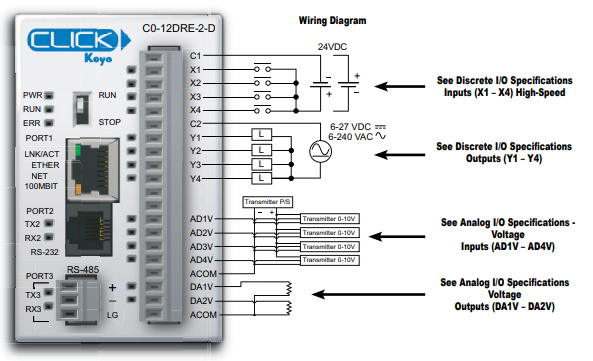
\includegraphics[width = 0.5\textwidth]{2_images/clickPlc}
            \caption{The Click \acrshort{plc} that has been used for the \acrshort{lmu}\cite{clickPlcData}.}
            \label{fig:plc}
        \end{figure} 
    
    \subsection{Remote I/O}
        Remote \acrshort{io} modules are responsible for controlling and monitoring the vast majority of \acrshort{io} onboard the lolly machine.
        Three ADAM Modules from Advantech were selected as the remote \acrshort{io} modules for the \acrshort{lmu}. The selection criteria for remote \acrshort{io} being much the same as that of the \acrshort{plc}: already used on campus, familiarisation among staff and Modbus TCP/IP compatibility. Other criteria for the distribution of \acrshort{io}  considered the type of \acrfull{io} devices onboard the lolly machine. Two types of remote \acrshort{io} modules have been selected for the \acrshort{lmu}, these are as follows:
        \begin{enumerate}
            \item \textbf{ADAM 6251} 16 Channel Digital Input Module
            \item \textbf{ADAM 6250} 8 Channel Digital Input/ 7 Channel Digital Output Module
        \end{enumerate}
    
        \begin{figure}[H]
        \centering
        \begin{minipage}{0.4\textwidth}
            \centering
            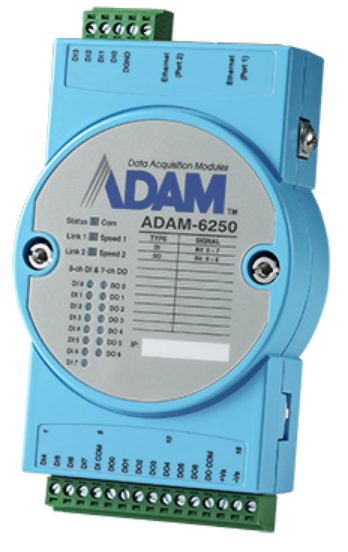
\includegraphics[width = 0.5\textwidth]{2_images/adam6250.png}
            \caption{6250 ADAM Module~\cite{6250Data}}
            \label{fig:adam6250}
        \end{minipage}\hfill
        \begin{minipage}{0.4\textwidth}
            \centering
            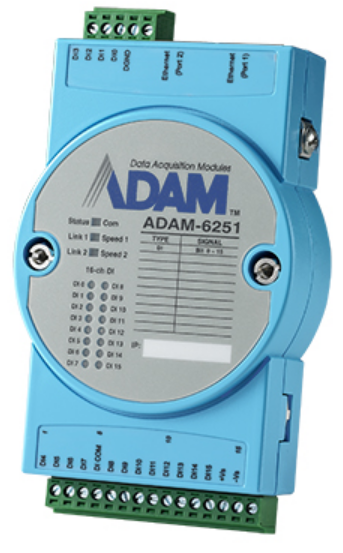
\includegraphics[width = 0.5\textwidth]{2_images/adam6251.png}
            \caption{6251 ADAM Module~\cite{6251Data}}
            \label{fig:adam6251}
        \end{minipage}\hfill            
        \end{figure}   
    
        More information about the ADAM modules can be found on the following web page links.
        
        \href{https://www.advantech.com/en-au/products/7447e150-338d-402d-b5a1-c9ce6d98816e/adam-6250/mod_da940b26-501f-413e-bfbc-732fd7496782}{ADAM-6250 "LINK"} \cite{6250Data} 
    
        \href{https://www.advantech.com/en-au/products/7447e150-338d-402d-b5a1-c9ce6d98816e/adam-6251/mod_98139b28-a181-4c45-83c9-01db52c3db7f}{ADAM-6251 "LINK"} \cite{6251Data} 
        

    \subsection{Siemens HMI}
        A Siemens KTP-600 Touch Panel is the main \acrshort{hmi} and has been permanently installed on the front of the lolly machine. The Siemens \acrshort{hmi} has been selected because it was already on campus and has the capability to communicate over Modbus TCP/IP. Specifics to how the \acrshort{hmi} functions is discussed in detail in Chapter \ref{chap:hmi}.
    
        \begin{figure}[H]
            \centering
            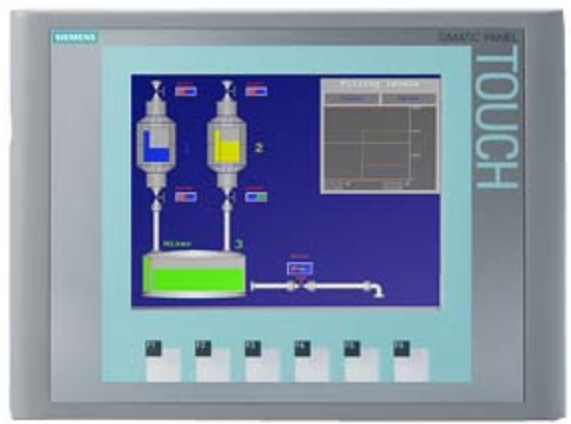
\includegraphics[width = 0.3\textwidth]{2_images/ktp600}
            \caption{The Siemens \acrshort{hmi} that has been used for the \acrshort{lmu}\cite{ktp600Data}.}
            \label{fig:hmi}
        \end{figure}
    
        More information about the Siemens \acrshort{hmi} can be found on the following web page link.
    
        \href{https://support.industry.siemens.com/cs/document/31032678/simatic-hmi-hmi-devices-basic-panels?dti=0&lc=en-WW}{KTP-600 Siemens HMI} \cite{ktp600Data} 
        
    
    \subsection{Raspberry Pi}
    A Raspberry-Pi microcontroller/ embedded PC has been setup as a wireless gateway for the lolly machine control system. The main function of the Pi is to host a program called NODE-RED which is an open sourced flow-based programming environment. For this project, Node-RED is used to interface a web based dashboard with the \acrshort{plc}. More information detailing the structure of the Node-Red flows is later discussed in Chapter /ref{chap:hmi}.
    
        \begin{figure}[H]
            \centering
            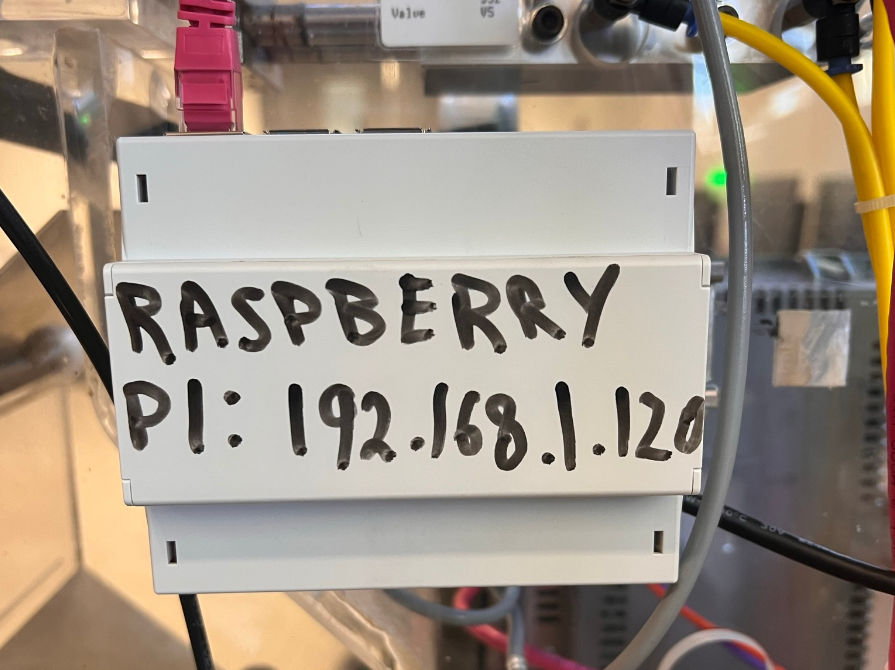
\includegraphics[width = 0.4\textwidth]{2_images/raspPiInstall}
            \caption{The Raspberry Pi that has been installed in the lolly machine.}
            \label{fig:raspPiInstall}
        \end{figure}
    
    
    \subsection{Arduino}
    An Arduino is used to control the \acrshort{rgb} light strip that surrounds the the front of the Lolly machine. This too is discussed later in the report in Chapter \ref{chap:hmi}. The Arduino has been setup with an RS-485 shield to allow instructions to be received form the \acrshort{plc}.
    
    \section{Physical/ Network Layer}
    
    \subsection{Overview}
    This section will discuss the type of networks that has been implemented on the \acrshort{lmu}. Various networks have been utilised trough the \acrshort{lmu} with Ethernet being the one used most extensively.
    
    \subsection{Ethernet} 
    The main backbone of all communications relies on an Ethernet network on the subnet: 192.168.1.X with a subnet mask of 255.255.255.0. Ethernet was selected as it an incredibly common communication medium that is used extensively throughout industry and also on campus. Physically, all devices are connected via an unmanaged network switch which is installed within the back of the Lolly Machine alongside the rest of the control gear. Pink Ethernet cables have been used to connect each device to one another for no other reason beyond pink being an awesome colour.
    
    \acrshort{ip} addresses are shown in the table below.	

        \begin{figure}[H]
            \centering
            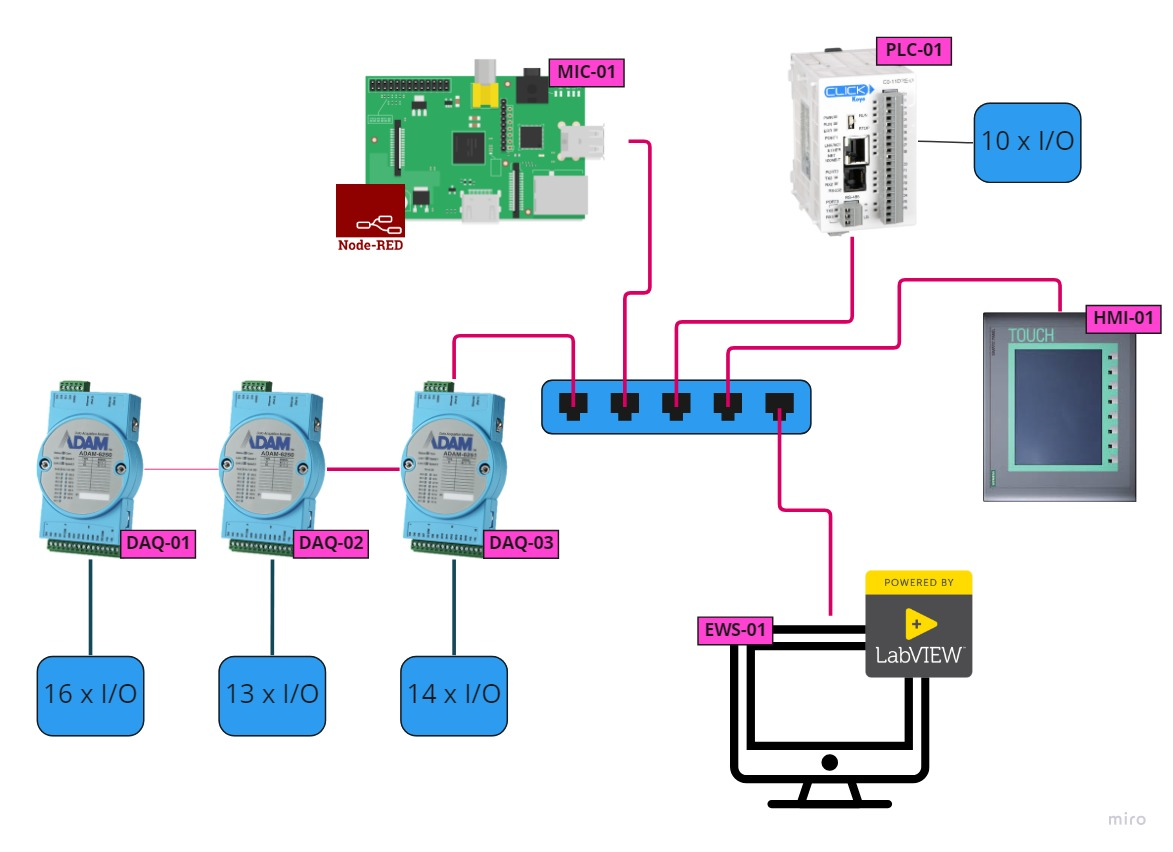
\includegraphics[width = 0.7\textwidth]{2_images/ethernetLollyMachine.png}
            \caption{The lolly machine Ethernet network.}
            \label{fig:ethernetLollyMachine}
        \end{figure}
    
    \subsection{WiFi}
    A WiFi network from the Raspberry Pi allows a remote connection from any device that is equipped with WiFi and a web browser. 
    
    \subsection{RS232}
    Unfortunately, the Click \acrshort{plc} does not come with a default \acrshort{ip} address. RS-232 is used to set the \acrshort{ip} address. Once the address is set, all other communication is archived via Ethernet as it is a superior in relation to RS-232.
    
    \subsection{RS485}
    RS-485 provides a communication interface between the \acrshort{plc} and the Arduino. RS-485 is not an essential network within the project as it is only responsible for changing the colours of the \acrshort{rgb} lights on the front side of the Lolly Machine.
    
    \subsection{SPI}
    The \acrshort{rgb} \acrshort{led}s controlled via the Arduino, are done so via the SPI serial communication protocol. A library has been written to control the \acrshort{rgb} \acrshort{led}s. The below link provides the source code located in a GitHub repository.
    
        \href{https://github.com/FastLED/FastLED}{FastLED source code "LINK"} \cite{FastLED} 
        
    \section{Software/ Application Layer}

    This section will discuss the hierarchy of control in regard to device to device communication. 
    The lolly machine is comprised of eight different network devices as detailed in Table \ref{table:networkDevices}

    \begin{table}[H]
        \caption{Network Devices}
        \begin{center}
            \begin{tabular}{|c|c|c|c|c|c|c|c|c|}
                \hline
                \textbf{Name} & \textbf{Manufacturer} & \textbf{Model} & \textbf{Type} & \textbf{Address}  & \textbf{Password}\\
                \hline
                DAQ-01 & Advantech & ADAM-6251 & Server & 192.168.0.20 & 00000000\\
                DAQ-02 & Advantech & ADAM-6250 & Server & 192.168.0.21 & 00000000\\
                DAQ-03 & Advantech & ADAM-6250 & Server & 192.168.0.22 & 00000000\\
                EWS-01 & NA & NA & Client & 192.168.0.113 & \\
                HMI-01 & Siemens & KTP-600 & Client & 192.168.0.15 & \\
                MIC-01 & Raspberry Pi & C0-12DRE-2-D & Client & 192.168.0.120 & raspberry\\
                MIC-02 & Arduino & UNO & NA & NA & \\
                PLC-01 & CLICK & C0-12DRE-2-D & Client-Server & 192.168.0.10 & click\\

                \hline
            \end{tabular}\\
        \end{center}
        \label{table:networkDevices}
    \end{table}
    
        \begin{figure}[H]
            \centering
            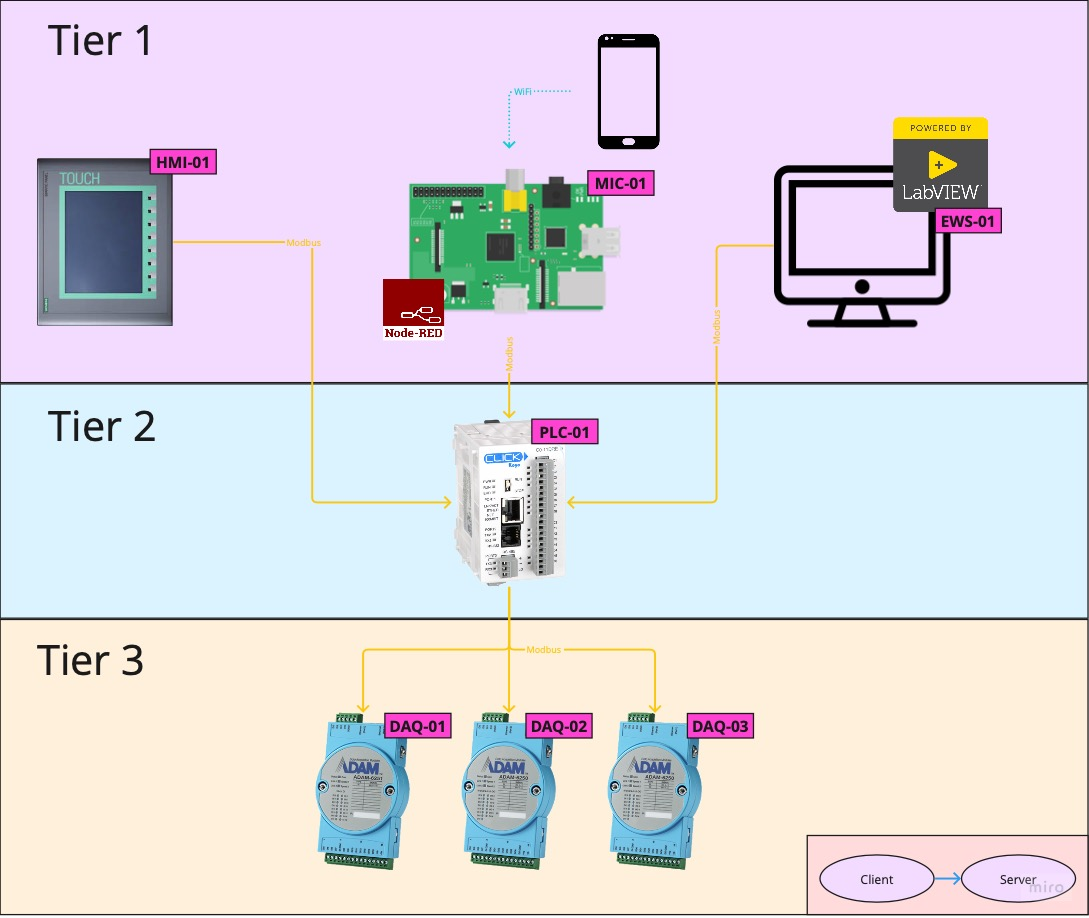
\includegraphics[width = 0.9\textwidth]{2_images/networkArcitecture.jpg}
            \caption{Overview of the lolly machine communication structure.}
            \label{fig:networkArcitecture}
        \end{figure}     
        


        The hierarchy of control, in regard to device-device communication, on the Lolly machine has been structured in a way that aims to facilitate a pragmatic, intuitive and robust method of communication between devices. The structure can be illustrated in a three tiered model where each tier is associated with a different communication function. All communication is achieved through Modbus TCP/IP over Ethernet with two exceptions which will be discussed later in Section \ref{sec:stripLed}.

        In a nutshell, the communication structure is pretty basic. Using terminology of a basic working relationship between a manager,  engineer and graduate,  the following can be applied to the communication structure of the Lolly Machine. A \acrshort{hmi} Client device (Tier 1) is the manager and tells the \acrshort{plc} Client-Server device (the engineer) what to do. The Engineer is responsible for doing some of her own work but is also in charge passing on certain tasks to the graduate. In the case of the Lolly Machine, it’s the same. The \acrshort{plc} is responsible for it’s own work but also passes some tasks down to the remote \acrshort{io} (graduate) in Tier 3. The remote \acrshort{io} is incapable of instructing the \acrshort{plc} what to do. 

        \subsection{Tier 1 - Client Devices}

        Tier 1 contains the Client devices. The main function of the client devices is to give instructions to the Server part of the \acrshort{plc}. The two main types of instructions to the \acrshort{plc} Server can be either read or write. A read instruction from a Client to a Server is a request for information. For example, an indicator on the Siemens \acrshort{hmi} that shows the status of a digital input, is “read” request from the \acrshort{hmi} to the \acrshort{plc}. When a Client writes to a server, in the case of the lolly machine, it is altering a value of an internal variable within the \acrshort{plc}. For example, In manual mode a request to turn on and off a digital output can be triggered by the \acrshort{hmi}.

        There are three different devices that act as Clients to the \acrshort{plc}. These are the: Siemens \acrshort{hmi}, Raspberry Pi (Node-RED) and the \acrshort{ews}(LabVIEW). The intention is that the Siemens \acrshort{hmi} will serve as the main control point, the \acrshort{ews} as a troubleshooting tool and the Raspberry Pi added as more of a novelty. The logic within the \acrshort{plc} responsible for mapping instructions from each of the Client devices will be discussed in Chapter \ref{chap:plc}.

        One other device that should get an honorary mention in this section is the optional device of a  phone/ tablet connected the Raspberry Pi \acrshort{wap}. In a matter of fact, the Raspberry Pi is actually a Client-Server device as it receives instruction from the connected phone/ tablet then proceeds to pass these commands onto the \acrshort{plc}. The reason that both devices have been left in tier 1 is because the Raspberry Pi doesn’t perform any logic. For the remainder of this document, the combination of both the devices will be referred to as the “Raspberry Pi”.

        \subsection{Tier 2 - Client-Server Devices}

        The only device in tier 2 is the \acrshort{plc}. The \acrshort{plc} is the central processor of the control system and is capable of receiving instructions from each of the \acrshort{hmi} Client devices and transmitting instructions to each remote \acrshort{io} Server devices. 

        \subsection{Tier 3 - Server Devices}

        Tier 3 contains Server devices. Server devices are only capable of receiving instruction from Client type devices (this includes Client-Server). All three remote \acrshort{io}s reside in tier 3. Although it is possible to control the Server devices in Tier 3 directly from tier 1 devices, this has not been done on this project. All communication is facilitated through the \acrshort{plc} in tier 2.




    
    
    
    
    \newpage
    
\chapter{Machine Program Development}
    \label{chap:plc}
    Programming the \acrshort{plc} was one of the largest tasks undertaken during the \acrshort{lmu} project. This task is multifaceted and includes design and implementation and is refereed to as ``Machine Program Development". This chapter discusses how the \acrshort{plc} has been programmed.

``CLICK Programming Software'' was used to program the \acrshort{plc}. The software is relatively basic in comparison to others that are currently available on the market. The simplistic nature of the software is great from a learning perspective, as the limited functionality allows new \acrshort{plc} programmers to become quickly acquainted with the software. The limited functionality also has it's downsides, the main one for this project being an inability to build custom functions, custom functions are useful when programming repetitive logic and would have been particularly helpful while programming some alarming logic - this will be discussed in section \ref{sec:replacePlc}. ``CLICK Programming Software'' is accessible for free through the following link - \href{https://www.automationdirect.com/clickplcs/free-software/free-click-software}{CLICK Software} \cite{clickSoftwareDownload}.


\section{I/O}
    For the \acrshort{plc} to be able to interact with the outside world, all \acrshort{io} needs to be configured and mapped. \acrshort{io} mapping is the process of setting up the \acrshort{plc} so that read (inputs) and write (outputs) addresses can be easily accessed throughout the program. 
    For this project, virtual \acrshort{io} refers to signals that do not have an association with anything physical on the machine while physical \acrshort{io} does. For example, an instruction to from the Siemens \acrshort{hmi} to the \acrshort{plc} would be considered virtual while an instruction from a push button is considered physical. The following practices have been implemented within the \acrshort{plc} \acrshort{ll} as method of ensuring standardisation throughout the code:
    
    \begin{enumerate}
        \item \acrshort{no} contacts within the \acrshort{ll} will be used to map virtual inputs from Client devices and will be read a maximum of one time within the program.
        \item \acrshort{ll} coil elements will be used to write to physical outputs and are to be written to a maximum of one time within the program. 
        \item Physical inputs are read as many times as necessary within the program and are implemented as \acrshort{no} contacts with the exception of the proximity sensors as they have \acrshort{nc} internal contacts. 
    \end{enumerate}

    All physical \acrshort{io} are terminated into either,  ADAM remote \acrshort{io} modules or directly into the \acrshort{plc} \acrshort{io}, typically refereed to as onboard \acrshort{io}.

    The following list provides a brief description for the various types of physical \acrshort{io} used on the lolly machine. These are referred to as \acrshort{io} tags.

    \begin{description}
        \item[V(k):] V = Valve, k = Valve number.
        \item[S(lm):] S = Position switch, l = associated valve, m = position switch number.
        \item[C(n):] C = Colour sensor, n = Sensor number.
    \end{description}



    \subsection{Onboard I/O}
        Onboard \acrshort{io} addresses can be found through the `System Configuration' window under the `Setup' tab. See Figure \ref{fig:plcConfig}
        Using onboard \acrshort{io} is a great deal easier than remote \acrshort{io} as configuration is quicker and easier - this will become evident in section \ref{sec:modbusClient}, where the Modbus \acrshort{io} mapping steps are discussed. Onboard \acrshort{io} are addressed as Xn for digital inputs and Yn for digital outputs where n = integer.
        
        \begin{figure}[H]
            \centering
            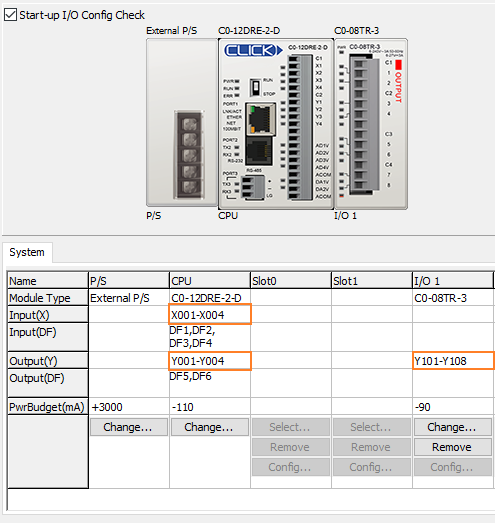
\includegraphics[width = 0.5\textwidth]{2_images/plcConfig.png}
            \caption{A screen shot of the `System Configuration' window of the PLC showing onboard I/O address.}
            \label{fig:plcConfig}
        \end{figure}
        
        The reason that all \acrshort{io} is not exclusively "onboard", is due to long lead times of \acrshort{plc} expansion modules. However, we were lucky enough to get one digital output module which is responsible for the \acrshort{led} status indicators on the front side of the Lolly Machine - three of which are in a traffic light arrangement which show the lolly machine status. A conscious decision was made to connect the status indicators directly to the \acrshort{plc} so the machine status can always be identified regardless of the communication health between devices. 

        \begin{figure}[H]
            \centering
            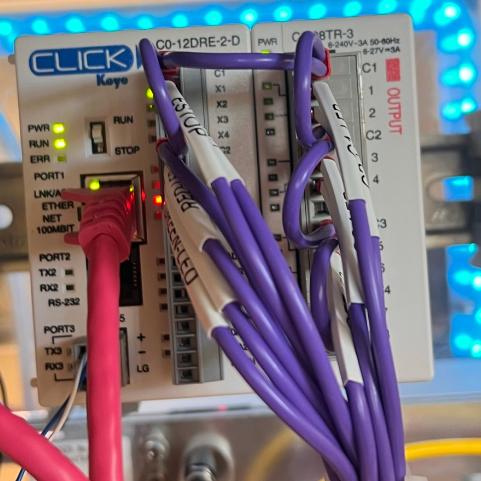
\includegraphics[width = 0.4\textwidth]{2_images/plcInstall}
            \caption{The Click PLC and expansion digital output module.}
            \label{fig:plcInstall}
        \end{figure}
    
    \subsection{Modbus I/O}
        Modbus \acrshort{io}, as the name suggests, are \acrshort{io} that are mapped to and from Modbus devices. As the \acrshort{plc} is a Client-Server device, there are two methods that must be discussed in regards to Modbus \acrshort{io} communication.

        \subsubsection{Server}
            The Modbus Server part of the \acrshort{plc} is accessible by Modbus Client devices. In the case of this project, these are the various control sources (\acrshort{hmi}s). Every variable within the \acrshort{plc} has an equivalent Modbus address which can be found within the `Address Picker' on the `Home' tab as illustrated by Figure \ref{fig:modbusAdd}. Next to the Modbus Addresses, are the function codes (see Table \ref{table:modbusFunctions}) that can be used to access the variable. There is no additional configuration that needs to be done to setup the \acrshort{plc} as a Modbus Server device. 
            
        \begin{figure}[H]
            \centering
            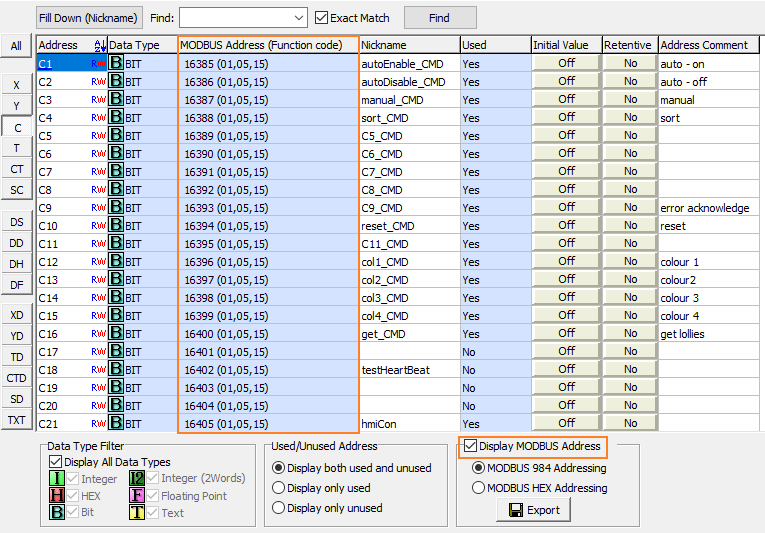
\includegraphics[width = 0.6\textwidth]{2_images/modbusAdd}
            \caption{Modbus Server addresses of the PLC.}
            \label{fig:modbusAdd}
        \end{figure}
        
            NOTE: Modbus address indexing can vary from device as some manufactures start from 0 while the others at 1. 
            
        \subsubsection{Client} \label{sec:modbusClient}
            The \acrshort{plc} Modbus Client is used to access the remote \acrshort{io} ADAM modules. Internal \acrshort{plc} addresses are linked to Server Modbus addresses of the ADAM modules through the use of receive and send functions within the \acrshort{plc}. Figure \ref{fig:plcModbusClient} shows the send and receive functions for DAQ-03. The receive function (top block of Figure \ref{fig:plcModbusClient}) is reading 8 bits of data (8 addresses) with a starting Modbus address of 01 and mapping then to internal Boolean variables, C232 to C240. The send function (middle block of Figure \ref{fig:plcModbusClient}), is writing to 7 Modbus address on DAQ-03, from 17 to 24 - these are driven by internal variables C240 to C247.

            A maximum of one communication function can be executed per \acrshort{plc} cycle. A counter is used to alternate between each communication function as illustrated in Figure \ref{fig:plcModbusClient} (bottom function).

        \begin{figure}[H]
            \centering
            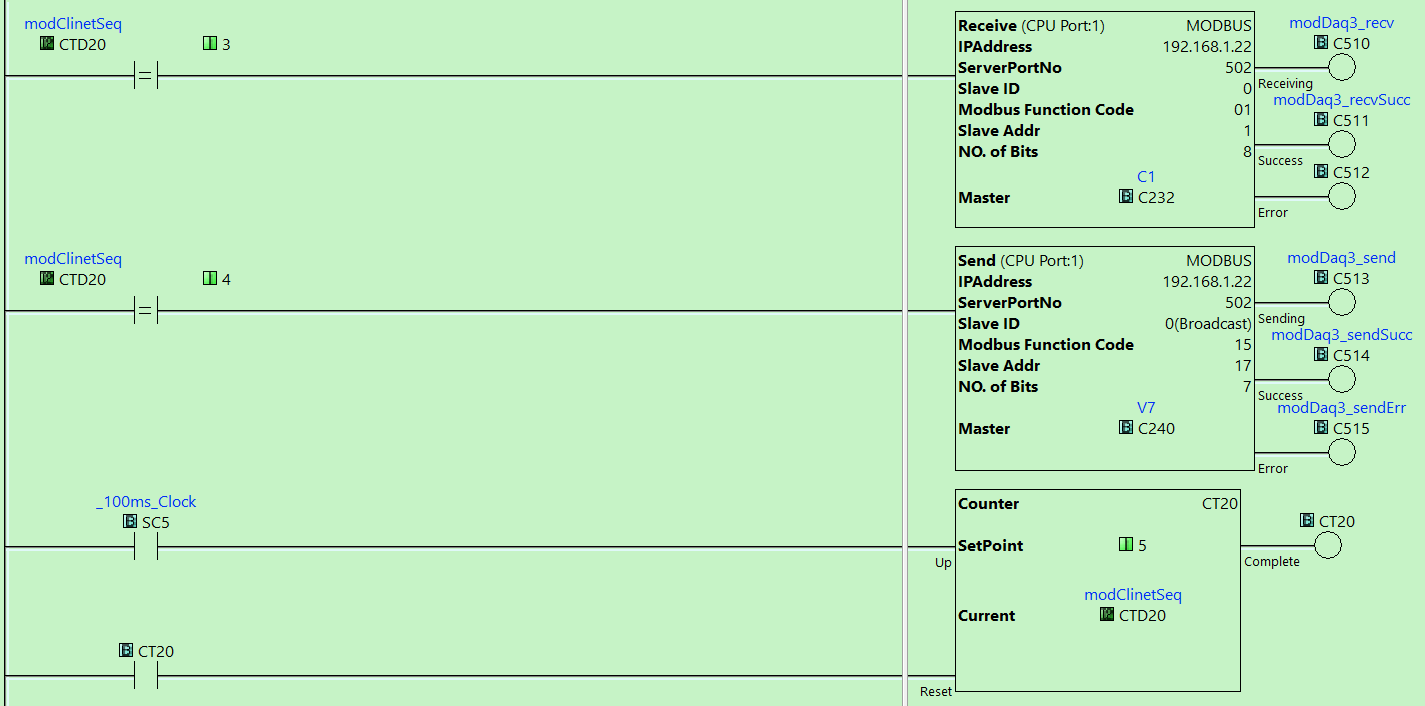
\includegraphics[width = 0.6\textwidth]{2_images/plcModbusClient}
            \caption{PLC Modbus Client send and receive functions within LL code.}
            \label{fig:plcModbusClient}
        \end{figure}
            
    \subsection{Input Mapping} \label{sec:input}
        Input mapping is almost exclusively concerned with virtual inputs from \acrshort{hmi} devices and can be found within the input subroutine program. The purpose of this portion of code is to define some logic that dictates which control source the \acrshort{plc} is taking instructions from. Figure \ref{fig:inputMapping}, for example, shows the three variables linked to each control source for the auto enable command - C1.
        \begin{description}
            \item C301 - Siemens \acrshort{hmi}
            \item C341 - LabVIEW application on \acrshort{ews} 
            \item C381 - Node-RED Dashboard running on the Raspberry Pi
        \end{description}
        
        Three internal variables dictate which control source the \acrshort{plc} is currently taking instruction from.
        \begin{description}
            \item C21 - Siemens \acrshort{hmi}
            \item C22 - LabVIEW application on \acrshort{ews}
            \item C23 - Node-RED Dashboard running on the Raspberry Pi
        \end{description} 
        So,for C1 to be True, the \acrshort{plc} must be taking instruction from the correct control source and the virtual input form the same control source must be true. After this is achieved, \acrshort{no} contacts linked with C1 can be easily used wherever necessary within the program. 

        Without this input logic, the \acrshort{plc} will attempt to receive instruction from all three control sources at once.
        
        \begin{figure}[H]
            \centering
            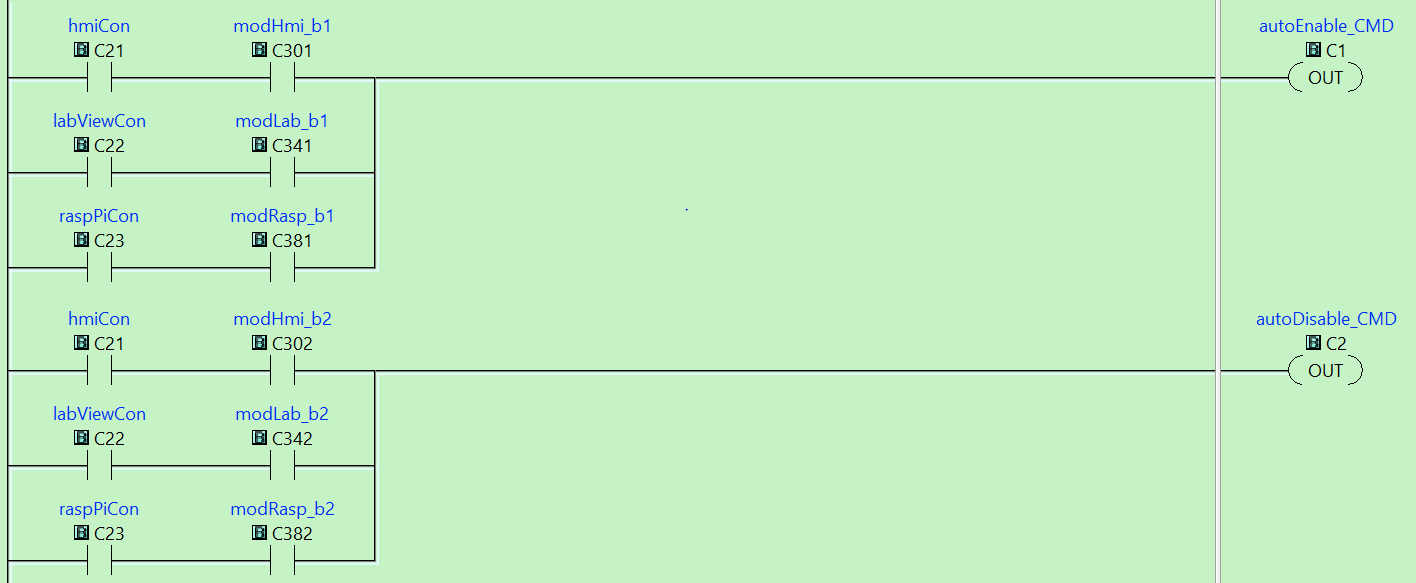
\includegraphics[width = 0.6\textwidth]{2_images/inputMapping}
            \caption{Input mapping from control sources.}
            \label{fig:inputMapping}
        \end{figure}
        
    \subsection{Output Mapping} \label{sec:output}
        Output mapping involves exclusively physical \acrshort{io} and consists of basic logic that dictates when outputs should be ON or OFF. When the device is in automatic mode, an internal variable driven from machine logic is linked to the output variable. When the machine is in manual mode, the variable associated with the selected control device is mapped directly to the output. 

        \begin{figure}[H]
            \centering
            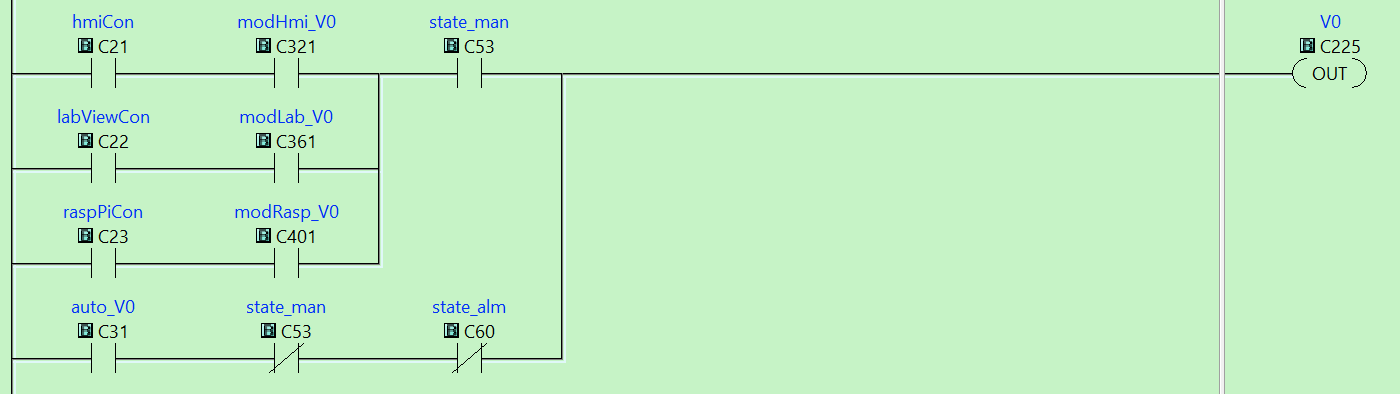
\includegraphics[width = 0.6\textwidth]{2_images/outputMapping}
            \caption{Output mapping to physical outputs.}
            \label{fig:outputMapping}
        \end{figure}        

\section{Machine Design and Implementation}
    The overall structure of the \acrshort{plc} code has been written in a modular style where program functions are split into separate subroutines. Subroutine programs are called from the main program as illustrated in Figure \ref{fig:plcMainAuto}. The main program is designed to be simple and easy to read. The only logic that exists within the main program is overall state machine which allows for the machine to be in one of three modes: Automatic, Manual or Alarm. A full printout of the \acrshort{plc} program can be found in Appendix \ref{app:plcProg}.

        \begin{figure}[H]
            \centering
            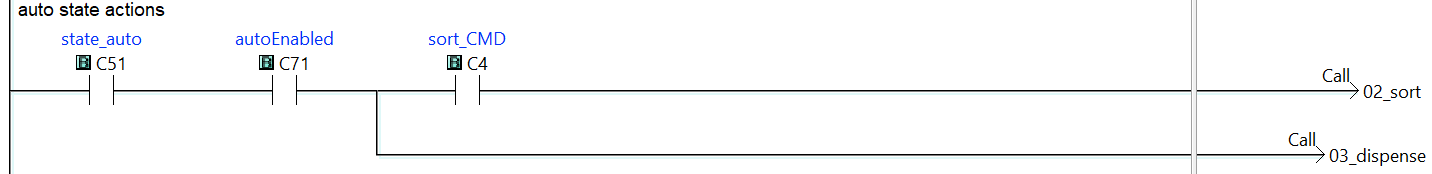
\includegraphics[width = 0.9\textwidth]{2_images/plcMainAuto}
            \caption{Snippet of PLC code showing where sort and dispense Subroutine Programs are called from the Main Program}
            \label{fig:plcMainAuto}
        \end{figure}
    The main program is also responsible for calling six other Subroutines Programs. This is achieved by connecting   ``\_Always\_ON'' \acrshort{no} contacts with each subroutine program.
    
    \subsection{Main Modes}
    A simplified version of state machine has been implemented for the structure the main program. A graphical representation of the program can be seen in Figure \ref{fig:mainStateMachine}. The machine will swap between manual and automatic mode as a function of the internal \acrshort{plc} variable C3. When an alarm becomes active, the system will go into `Alarm Mode' regardless of whether the machine is in manual or automatic. 
    
        \begin{figure}[H]
            \centering
            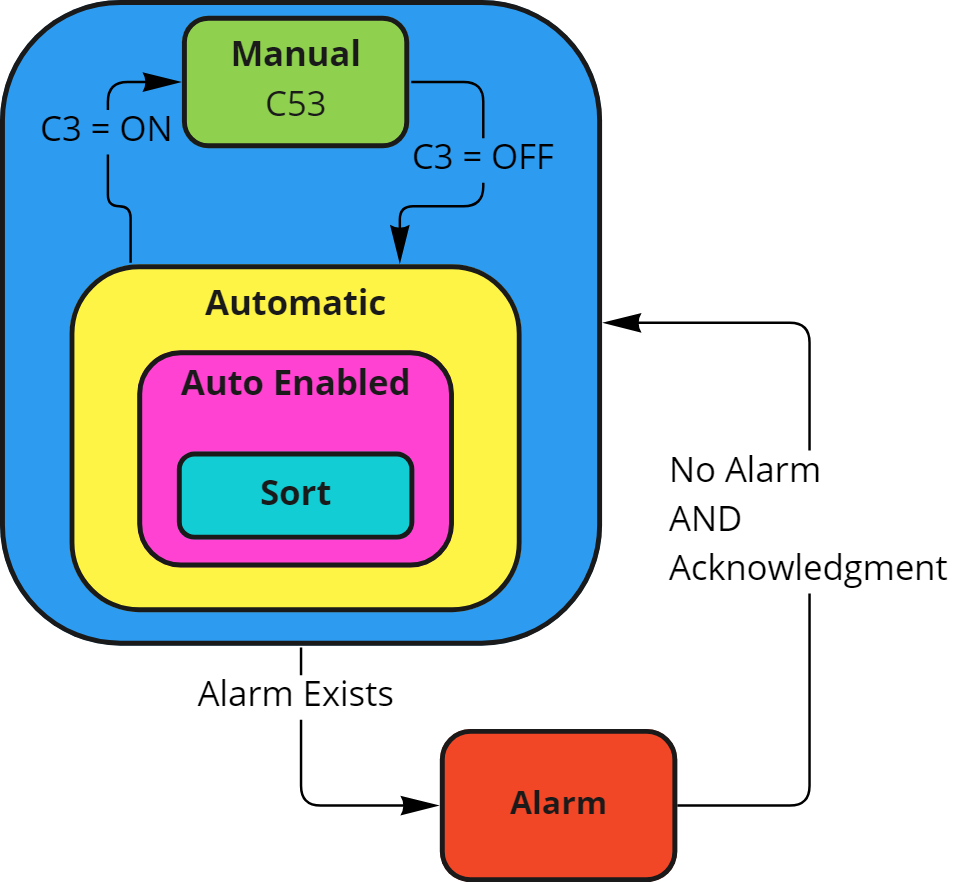
\includegraphics[width = 0.3\textwidth]{2_images/mainStateMachine}
            \caption{State machine design for the main program.}
            \label{fig:mainStateMachine}
        \end{figure}
    
        \subsubsection{Automatic}
            When C3 is off and the machine is not in an alarm state, the machine will be in automatic mode. For the system to function in automatic mode, it must be enabled.  Once enabled, the dispense subroutine program is called. The sort subroutine is called when automatic mode is enabled and C4 is ON. The reason that these two subroutines are not called at the same time is to allow the machine to dispense lollies while it is not sorting. 
            When the machine initially goes into automatic mode, the green \acrshort{led} status indicator will flash. When the machine is enabled in automatic mode the green \acrshort{led} will become solid.

        \subsubsection{Manual}
            When C3 is on and the machine is not in an alarm state, the machine will be in manual mode. While in manual mode, control valves can be manipulated via the connected control source. The logic that drives the manual control is detailed in Section \ref{sec:output}.
            When the machine is in manual mode, the amber \acrshort{led} status indicator will be on. 

        \subsubsection{Alarm}
            When an alarm is present, the machine will go into alarm mode. While in Alarm mode, the machine will be inoperable and outputs will go back to their default position. When the machine is in alarm mode, the red \acrshort{led} status indicator will be on.

    \subsection{Dispensing}
        Dispensing is a function of the lolly machine which is possible when the machine is enabled in automatic mode. While in this mode, the machine is constantly waiting for an input from the user which dictates what colour/s of lolly to dispense. Once the user has selected what colour lollies they want, they presses the get button and the machine will dispense the lollies. This function has been coded using general ladder logic programming principles and can be found in Appendix \ref{app:plcProg}. State machine design was considered but not implemented to to the simplicity of this function. 
        
    \subsection{Sort}
        The sorting subroutine is the most complex piece of code within the controller and has been written exclusively in state machine. The basic process flow is as follows. 

        \begin{enumerate}
            \item A lolly is transferred from the primary hopper into the colour detection shoot.
            \item The lolly colour will be detected and the colour paddles will move into position.
            \item The lolly will drop into the secondary hopper associated with the detected colour.
            \item Repeat.
        \end{enumerate}

        If the colour cannot be detected then the lolly is recycled back into the primary hopper via the reject hopper and shoot. 

        An illustration of the state machine design shown in Figure \ref{fig:sortStateMachine} provides a detailed view of all possible actions and transitions within the sorting program.


        \begin{figure}[H]
            \centering
            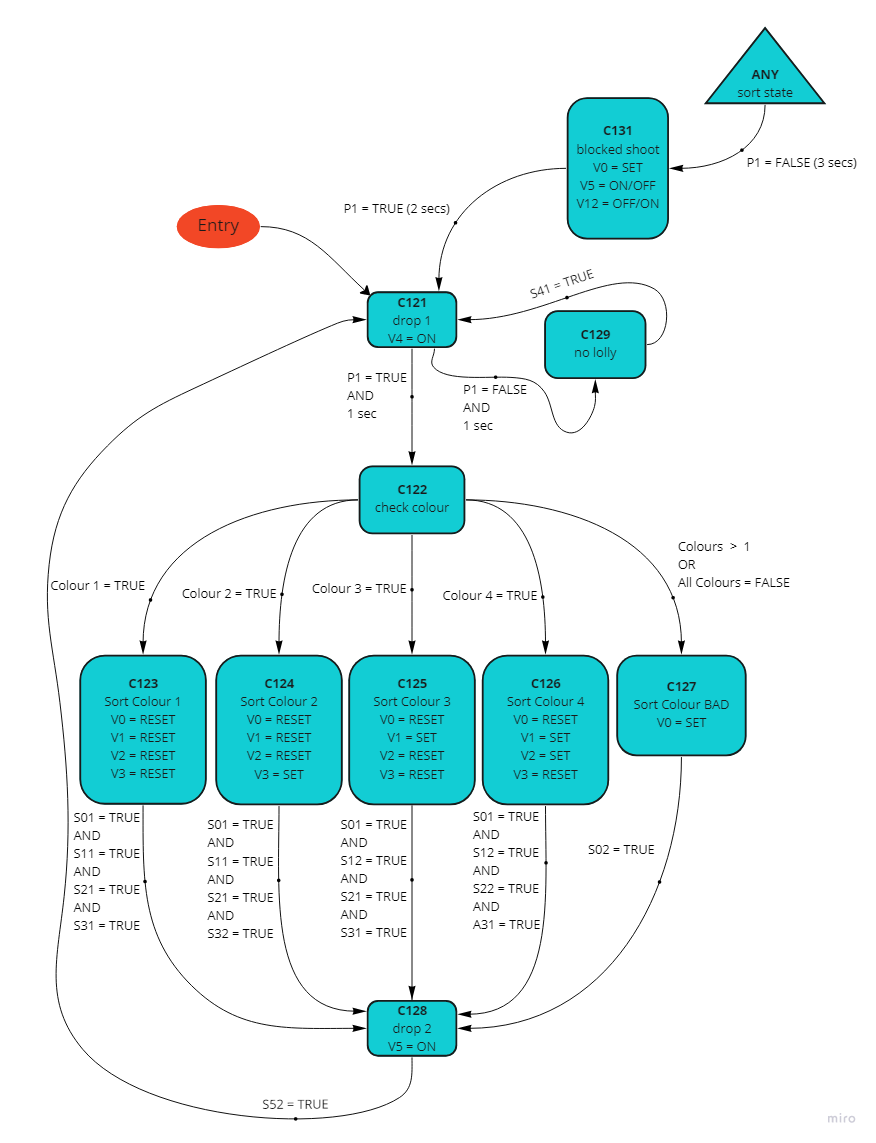
\includegraphics[width = 0.6\textwidth]{2_images/sortStateMachine}
            \caption{State machine design for the sorting program.}
            \label{fig:sortStateMachine}
        \end{figure}
        
    \subsection{Alarm Mode}
        An alarm subroutine program contains logic for alarm functions. There are 21 different conditions that will put the machine into alarm mode. Two words (See Table \ref{table:dataTypes}) are used to determine the specific nature of the alarm where each bit within each word is associated with a different alarm. A 16-bit  addresses represents the word within the \acrshort{plc}. To turn on individual bits within the 16 bit integer, the value of the corresponding bit is added to running total when the alarm is activated. Figure \ref{fig:alarmWord} below shows that when a \acrshort{ftc} alarm for V0 occurs, 2 is added to `alarmWord1'. The bit within `alarmWord1' corresponding to this alarm is bit number 2. 2 = 0000000000000010 .
        Alarm words a reset by changing the value back to zero. 

        \begin{figure}[H]
            \centering
            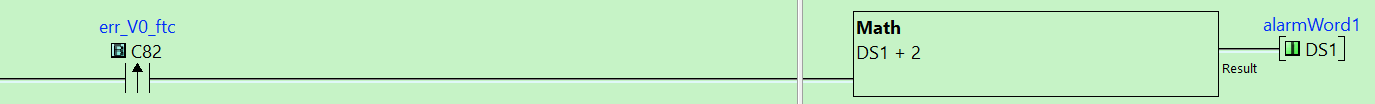
\includegraphics[width = 0.6\textwidth]{2_images/alarmWord}
            \caption{LL showing how alarm words are generated.}
            \label{fig:alarmWord}
        \end{figure}

\section{Special Functions}
    Special functions are those that are not necessary for the basic operation of the lolly machine but do add value to the overall function of the machine.

    \subsection{Automatic Shoot Unblock}
        Sometimes, when a lolly is transferred from the primary hopper into the colour detection shoot, the proximity sensor that detects the presence of a lolly does not register that a lolly is in situ. When this happens, another lolly will be dropped into the shoot. This can often lead to a lolly jam and the machine will continue to drop lollies - even if the shoot is blocked. To combat this, the automatic shoot unblock function has been added into the sorting program. 
        During normal operation with the sorting program running, there should never be a lolly in the color detection shoot for longer than two seconds. 
        Logic has been included that will pause the sorting process and activate the automatic shoot unblock function whenever the proximity sensor that detects the presence of a lolly is obstructed for longer than three seconds. While the function is active, pressurised air is directed into the shoot while V5 alternates between positions. The combination of the pressurised air and a moving base(V5) works surprisingly well to dislodge stuck lollies. The unblocking function is active until the shoot is cleared. This section of code can be found in Appendix \ref{app:plcProg} within the sorting subroutine. 
        
        Just as a side note, the reason the machine will attempt to drop an additional lolly if none are detected is because sometimes a lolly does not fall into the colour detection shoot when V4 actuates between positions. 

    \subsection{Automatic Control Source Recovery} \label{sec:autoConRec}
        Automatic control source recovery is a function that automatically connects to an alternative control source when connection from the active control source is lost. For this function to work, the \acrshort{plc} must be able to detect when communication is healthy and unhealthy. In this project, communication status is detected through two separate methods. 

        \begin{description}
        
            \item[Heart Beat:] A heart beat is a periodically alternating Boolean signal that is produced by one device and received by another. The receiving device infers a healthy connection when the signal alternates within a given time, i.e., when the heart beat stops, communication is unhealthy. 
            
            \item[Watch Dog:] A watchdog timer repetitively increments up to a predefined value. The timer value is produced by one device and received by another. An unhealthy connection between devices is registered when the receiving device doesn't detect a change in value for a given period.
            
        \end{description}

        Communication status of the Siemens \acrshort{hmi} is detected by a heartbeat signal within a status word while the Node-RED and LabVIEW program both utilise a watchdog timer. The Siemens heart beat is built into the configuration of the device while the watchdog timers for Node-RED and LabVIEW needed to be coded into the program.
        \acrshort{ll} code shown in Figure \ref{fig:autoControlSourceRecovery} illustrates how the \acrshort{plc} automatically establishes a new connection when communication is lost from the current control source.  

        \begin{figure}[H]
            \centering
            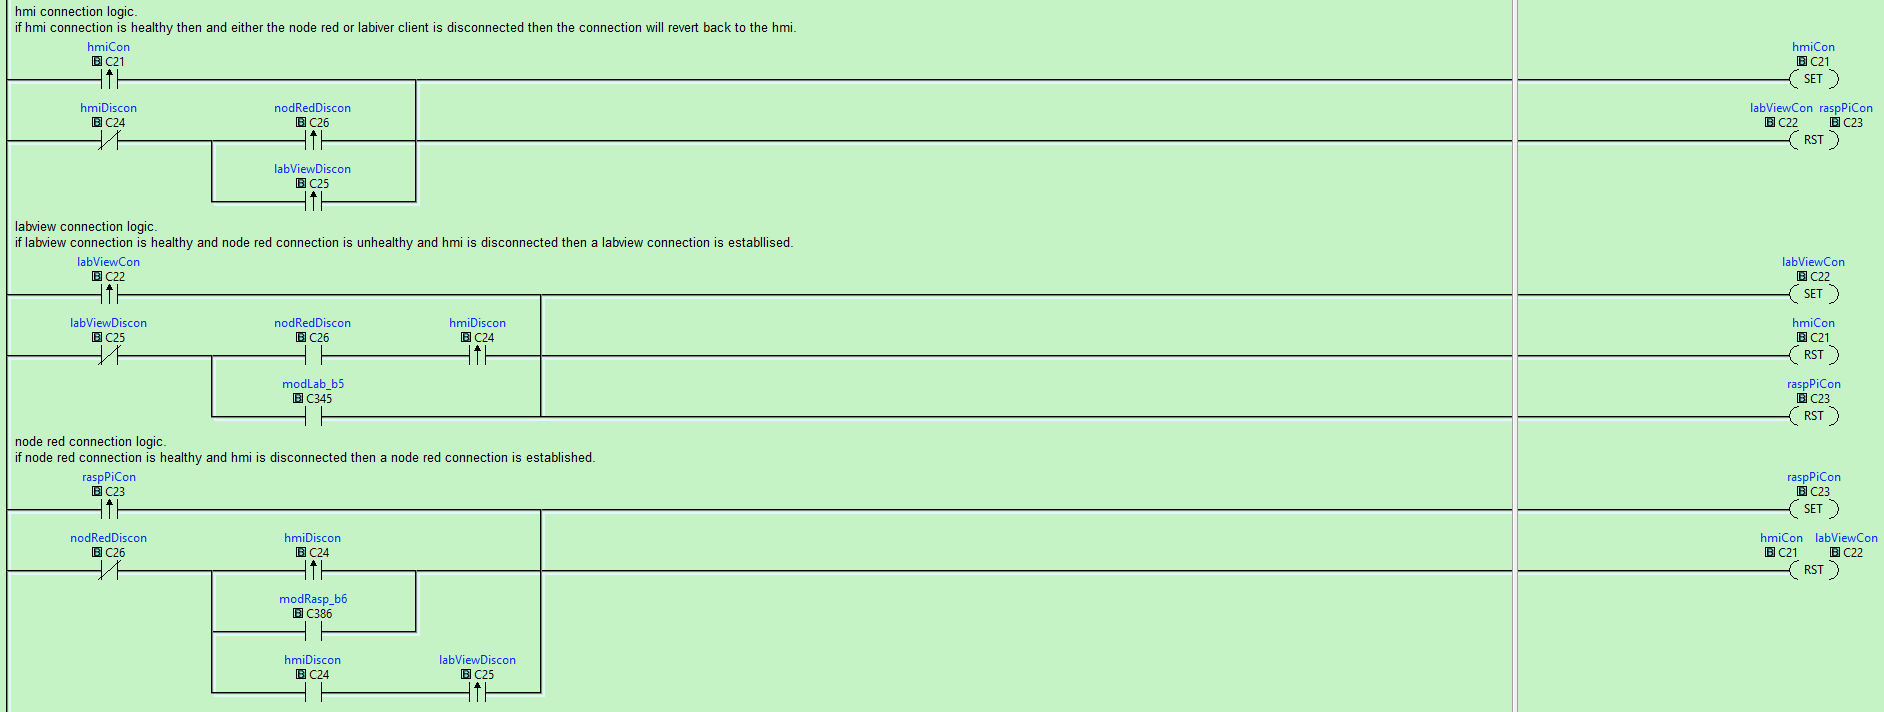
\includegraphics[width = 0.6\textwidth]{2_images/autoControlSourceRecovery}
            \caption{LL showing the automatic control source recovery.}
            \label{fig:autoControlSourceRecovery}
        \end{figure}        

    \subsection{Valve FTO/ FTC} \label{sec:valveFtoFtc}
        \acrfull{fto} and \acrfull{ftc} logic puts the machine into alarm mode in the event that a valve either fails to open or fails to close. The idea that drives this function is pretty basic, if a valve is given an instruction to either open or close, and it does not, then a \acrshort{fto} or \acrshort{ftc} alarm will become active. This function is achieved by comparing the status of the output driving the valve with the inputs from the valve position sensors. If the sensor does not detect the correct valve position after two seconds then an alarm is activated. \acrshort{fto} and \acrshort{ftc} code was particularly cumbersome to write as the \acrshort{plc} software does not support custom functions, this is discussed in more detail in the future recommendations Section \ref{sec:replacePlc}.

        \begin{figure}[H]
            \centering
            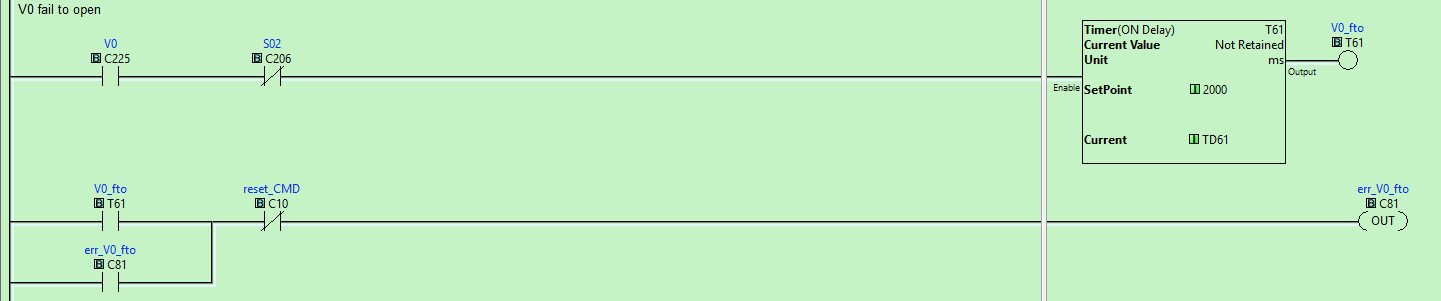
\includegraphics[width = 0.6\textwidth]{2_images/ftoLl}
            \caption{LL of FTO logic for V0.}
            \label{fig:ftoLl}
        \end{figure}          
        This function is capable of working in both automatic and manual mode.   
        
    \subsection{Strip LED on Front Surround} \label{sec:stripLed}
        An \acrshort{rgb} \acrshort{led} strip that surrounds the front of the machine has been programmed to change colour whenever a lolly is dropped into the colour detection shoot. The \acrshort{rgb} colour matches that of the lolly. This is achieved through the use of an Arduino microcontroller and the RS-485 communication port of the \acrshort{plc}. When a new colour is detected, an RS485 signal is transmitted from the \acrshort{plc} and received by the Arduino. The Arduino then controls the \acrshort{led} strip through a communication protocol called \acrshort{spi} \footnote{For more information about \acrshort{spi} click this \href{https://learn.sparkfun.com/tutorials/serial-peripheral-interface-spi/all}{link.} \cite{spi}}. Appendix \ref{app:arduino} contains the code within the Arduino.

        \begin{figure}[H]
            \centering
            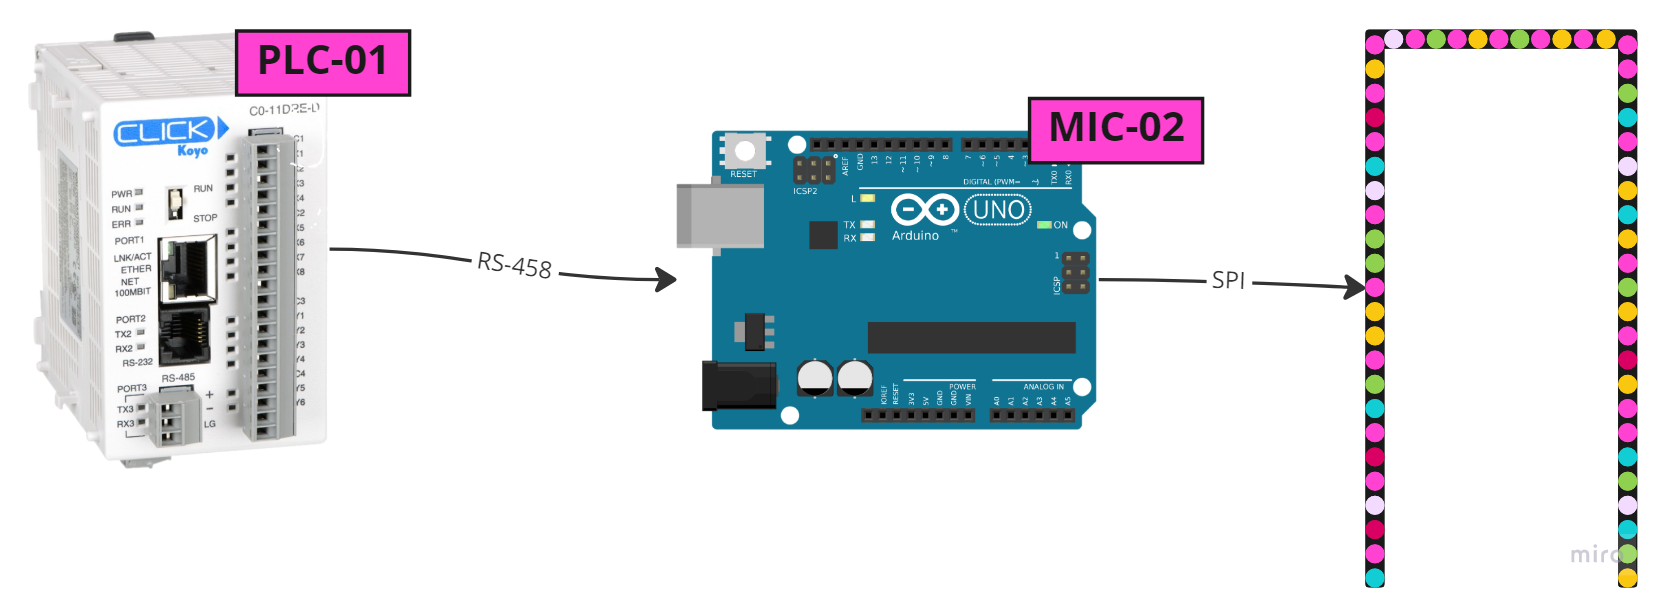
\includegraphics[width = 0.6\textwidth]{2_images/rgbStrip}
            \caption{Communication flow between the PLC and RGB LED strip.}
            \label{fig:rgbStrip}
        \end{figure} 
    \newpage  
    
\chapter{HMI Development}
    \label{chap:hmi}
    Three \acrshort{hmi}s have been configured and programmed as control sources for the lolly machine. This chapter provides detail into \acrshort{hmi} development. All \acrshort{hmi}s communicate with the \acrshort{plc} through Modbus \acrshort{tcpIp}.

\section{Siemens HMI}
    A KTP600 Siemens \acrshort{hmi} is the main control source and is permanently mounted to the front of the machine. The KTP600 is a touch screen device accompanied by six push buttons.  This \acrshort{hmi} serves as a setup and diagnostic tool for operators as well as an interface for machine users on open days. With many users being children, a main design consideration was that user screens needed to be functionally simplistic with a `fun' feel. The layout of the screens will be discussed further in Section \ref{sec:hmiScreens}. Programming the KTP600 was done using \acrfull{tia} Portal by Siemens.

        \begin{figure}[H]
            \centering
            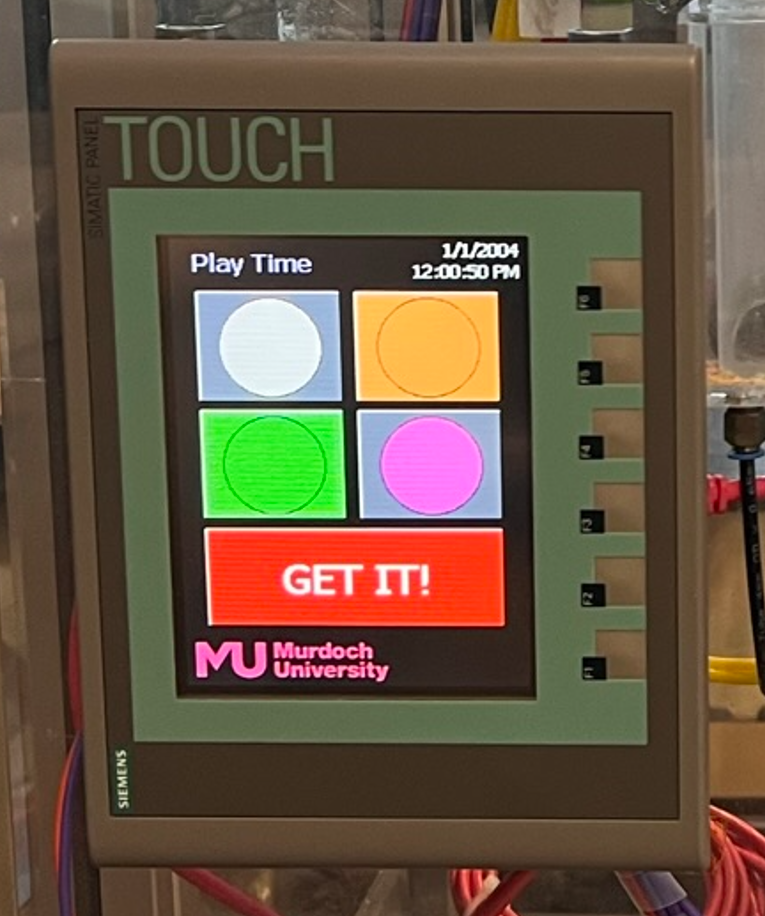
\includegraphics[width = 0.45\textwidth]{2_images/hmiInstalled}
            \caption{The Siemens HMI showing the Play screen.}
            \label{fig:hmiInstalled}
        \end{figure}    
    
    \subsection{Configuration}
        \subsubsection{Modbus Communication}
            To allow communication between the \acrshort{hmi} and the \acrshort{plc}, a connection must be added and configured within the \acrshort{hmi}. Figure \ref{fig:modbusHmiConfig} shows the configuration for the Modbus connection between the \acrshort{hmi} and \acrshort{plc}. Once a Modbus connection is added and configured, \acrshort{hmi} tags need to be defined. \acrshort{hmi} tags are address links between the \acrshort{hmi} and the \acrshort{plc}. Objects (buttons, indicators, etc) on the \acrshort{hmi} screens are linked to tags with read and/or write access. 
            
        \begin{figure}[H]
            \centering
            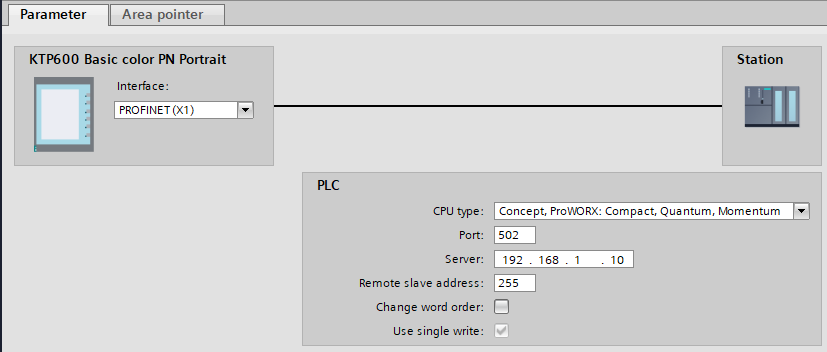
\includegraphics[width = 0.5\textwidth]{2_images/modbusHmiConfig}
            \caption{Configuration settings for a Modbus connection within the Siemens HMI.}
            \label{fig:modbusHmiConfig}
        \end{figure}        
        
        \subsubsection{Alarms}
            Two alarm Words transmitted from the \acrshort{plc} provide the \acrshort{hmi} with 21 different discrete alarms where each bit within each word is associated with a different alarm. Discrete alarms are made up of a trigger tag and a trigger bit. The tag is the alarm Word and the trigger bit is the index of the bit within the alarm word. This is illustrated in Figure \ref{fig:hmiAlarms}.

        \begin{figure}[H]
            \centering
            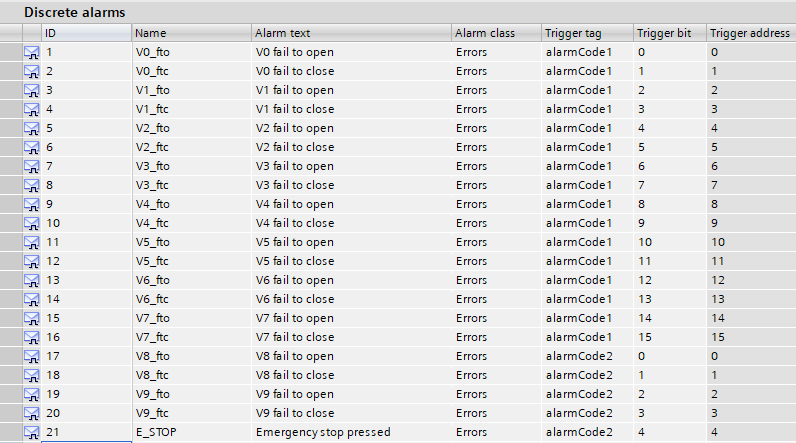
\includegraphics[width = 0.6\textwidth]{2_images/hmiAlarms}
            \caption{Alarm configuration of the Siemens HMI.}
            \label{fig:hmiAlarms}
        \end{figure}    

         When an alarm occurs, a popup containing alarm details will appear on the \acrshort{hmi}. To reset the alarm, the F1 (reset) button must be pressed. To clear the popup the ! button must be pressed. Figure \ref{fig:hmiAlarm} provides an example of what an alarm looks like on the \acrshort{hmi}.

        \begin{figure}[H]
            \centering
            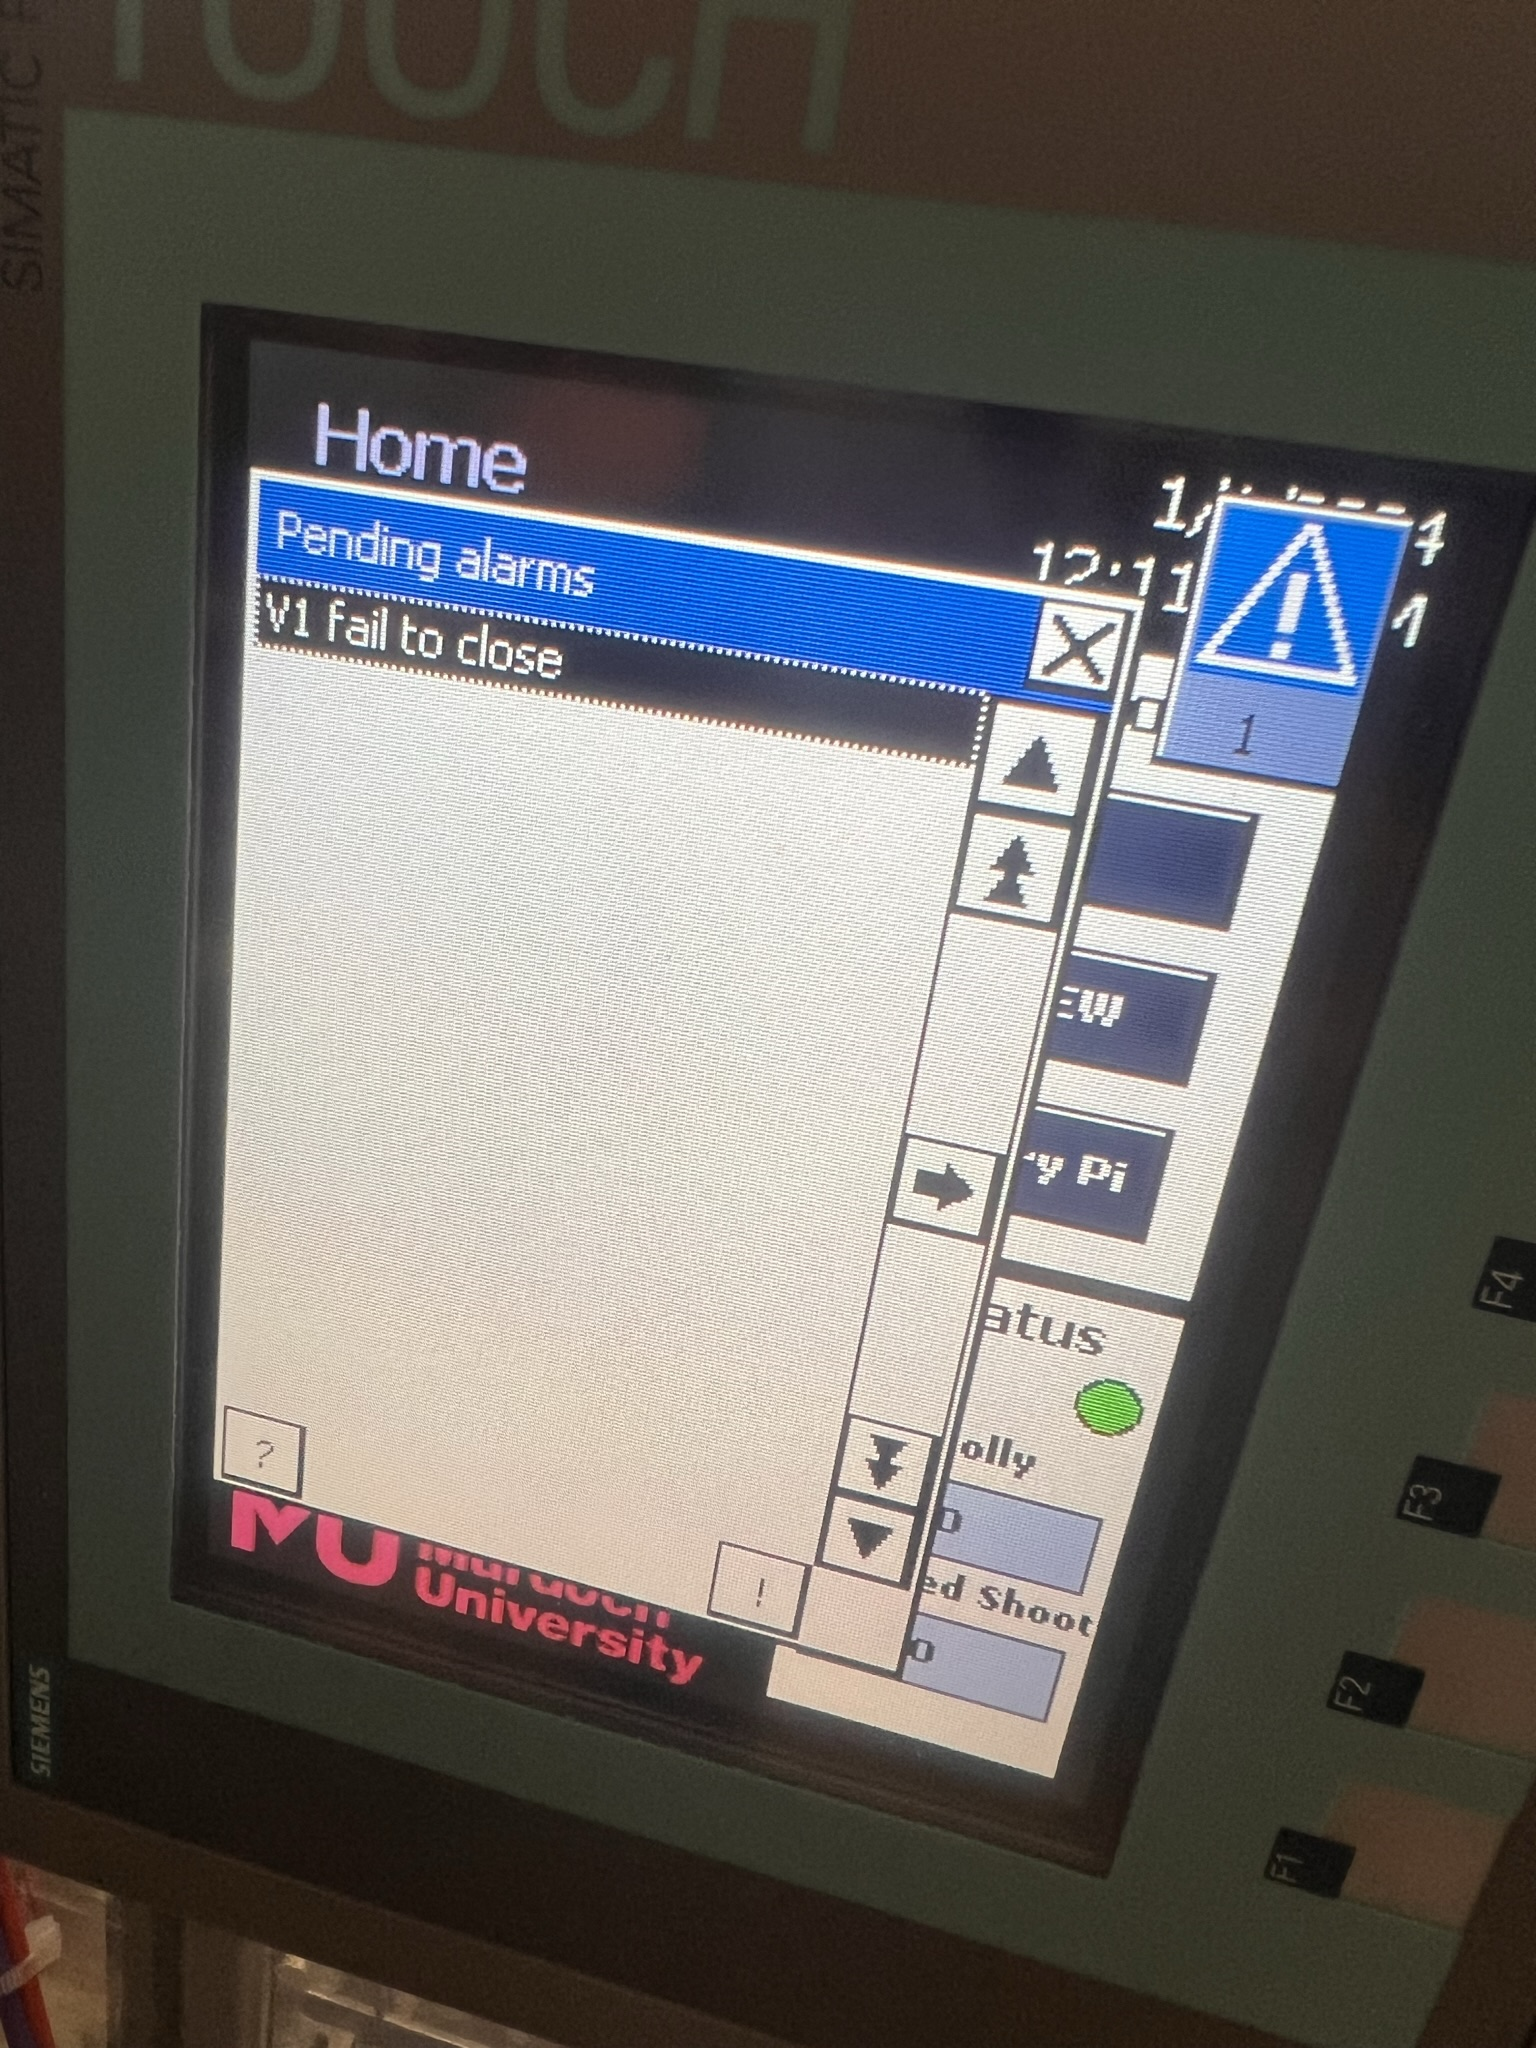
\includegraphics[width = 0.3\textwidth]{2_images/hmiAlarm}
            \caption{V1 fail to close alarm.}
            \label{fig:hmiAlarm}
        \end{figure}  
            
        \subsubsection{Heart Beat}
            The heartbeat from the Siemens \acrshort{hmi} is produced by a status word which Siemens refer to as the coordination area pointer. The second bit of the coordination area pointer is the `Life Bit' which is used as the heartbeat signal to the \acrshort{plc}. The coordination area pointer is linked to a Modbus address within the configuration connection.
            The startup bit and operation mode bits are not used within this project. 

        \begin{figure}[H]
            \centering
            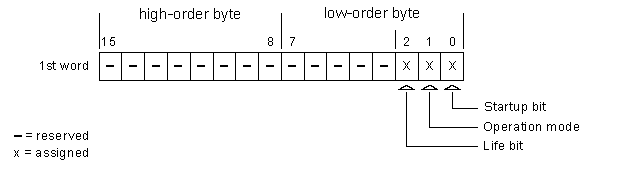
\includegraphics[width = 0.6\textwidth]{2_images/hmiCoordination}
            \caption{Coordination area pointer bit assignment\cite{tiaManual}}
            \label{fig:hmiCoordination}
        \end{figure} 
            

    \subsection{Screens} \label{sec:hmiScreens}
        Four screens provide user interfaces for configuration, diagnostics and general users who just want lollies. Six F keys on the right of the screen have been configured with various functions these are as follows:

        \begin{description}

        \item[F1:] Go to home screen
        \item[F2:] Go to play screen
        \item[F3:] Spare 
        \item[F4:] Spare
        \item[F5:] Toggle sorting program
        \item[F6:] Reset/ acknowledge alarms
        
        The `F' keys have been intentionally left unlabeled to discourage younger users from pressing the buttons. 
        Operation of the Siemens \acrshort{hmi} is outlined in the user manual in Appendix \ref{app:userGuide}
        
        \end{description}

        \subsubsection{Play}
        The play screen (Figure \ref{fig:hmiPlay}) has been specifically designed for users on open days. The main design consideration for this screen was to make it as simplistic as possible to allow operation from young users. 
        To use the play screen, the machine must be enabled in automatic mode. This screen is linked to the dispensing function of the machine.  The play screen can be accessed from the home screen by pressing the `Play' button or by pressing F5. 
        
        \begin{figure}[H]
            \centering
            \includegraphics[width = 0.3\textwidth]{2_images/hmiPlay}
            \caption{The Play screen on the Siemens HMI}
            \label{fig:hmiPlay}
        \end{figure} 

        \subsubsection{Home}
            The home page is the main screen from a machine operations and maintenance perspective. This screen allows the operator to control and monitor the machine mode and control source - it also provides navigation to other screens. This screen can be accessed by at any time by pressing F1.  
        
        \begin{figure}[H]
            \centering
            \includegraphics[width = 0.3\textwidth]{2_images/hmiHome.png}
            \caption{The home screen on the Siemens HMI}
            \label{fig:hmiHome}
        \end{figure} 
        
        \subsubsection{Manual}
            This screen provides manual operation to all valves. To change the state of a valve in manual mode, simply press the Vn button. When the valve is switched on the grey button will change color to green. This screen is accessible by pressing the manual button on the home screen. 

        \begin{figure}[H]
            \centering
            \includegraphics[width = 0.3\textwidth]{2_images/hmiManual}
            \caption{The manual screen on the Siemens HMI}
            \label{fig:hmiManual}
        \end{figure} 

        \subsubsection{IO}
            This screen shows machine \acrshort{io} status. This screen can be used as a diagnostic tool for machine operators. The \acrshort{io} screen also provides an impressive representation of the events occurring while the sorting program is running and users are dispensing lollies. This screen will show the \acrshort{io} status regardless of which control source is active.   

            \begin{description}
                \item Grey = False
                \item Green = True
            \end{description}

        \begin{figure}[H]
            \centering
            \includegraphics[width = 0.3\textwidth]{2_images/hmiIo}
            \caption{The io screen on the Siemens HMI}
            \label{fig:hmiIo}
        \end{figure} 
    
\section{LabVIEW}
    A LabVIEW application to control and monitor the lolly machine has also been developed. This interface has been built with an intuitive design to allow operators to easily troubleshoot and diagnose problems. The LabVIEW application was the quickest to develop as functions from inbuilt libraries were used for most programming tasks.

    While developing with LabVIEW, the front and back panel are developed at the same time - this makes development comparatively quick.
    
    \subsection{Back Panel}
    
        The back panel of the LabVIEW program contains program logic and functions that drive the application. 
        
        \subsubsection{Modbus Communication}
        
            Modbus communication functions from \href{https://www.ni.com/en-au/support/downloads/tools-network/download.modbus-master.html#374378}{Modbus Master by Plasmionique Inc.} made configuring and programming Modbus components a uncomplicated task \cite{modbusLabview}.
            
            Establishing a connection to the \acrshort{plc} is accomplished through a Modbus master function which requires the \acrshort{ip} address and port number of the Modbus server - the \acrshort{plc}(192.168.1.10). 
            Read functions (reading glasses) are used to read values form the Modbus Server while write functions (pencil), write values to the Server. Address indexing in LabVIEW starts at zero while the \acrshort{plc} starts at one, this means that an offset of one exists between Modbus addresses of the \acrshort{plc} and the LabVIEW application. Figure\ref{fig:modLabFun}
            
        \begin{figure}[H]
            \centering
            \includegraphics[width = 0.9\textwidth]{2_images/labViewModFunc}
            \caption{The Modbus functions on the LabVIEW back panel.}
            \label{fig:modLabFun}
        \end{figure}     
        
        \subsubsection{Watch Dog Timer}
            Building a watchdog timer with LabVIEW was a simple task with the core components being the loop iteration number and a quotient/ remainder function. An additional feature is added to the watchdog timer that allows users to pause the timer. This feature is included to simulate a disconnection, thus, demonstrating the  previously discussed automatic control source recovery function (Section \ref{sec:autoConRec}).

        \begin{figure}[H]
            \centering
            \includegraphics[width = 0.2\textwidth]{2_images/labFrontWatchDog}
            \caption{The LabVIEW watchdog indicator.}
            \label{fig:labFrontWatchDog}
        \end{figure}    
            
            
        \subsubsection{Data Conversion}
            To read data from the \acrshort{plc}, data needed to be converted from a Boolean array into individual bits, and vice versa for writing. This was achieved in LabVIEW using standard array functions found in the main tool palette. Converting the alarm words into individual bits was accomplished through a few different functions. An array of 16 bit integers is split into two separate integers. Each integer is then converted into bits which are connected to Boolean indicators. This flow of conversions is illustrated in Figure \ref{fig:labViewAlarmUnmap}.

        \begin{figure}[H]
                \centering
                \includegraphics[width = 0.4\textwidth]{2_images/labViewAlarmUnmap}
                \caption{Unmapping alarm words with LabVIEW.}
                \label{fig:labViewAlarmUnmap}
        \end{figure}   
            
        \subsubsection{Front Panel}

            The front panel of the LabVIEW application is what the users interact with.
            
            The LabVIEW front panel for this project has been designed to look like the machine. The intention behind this was to make troubleshooting and diagnostics activities more intuitive and therefore a quicker and easier. Although LabVIEW has the capability to build complicated screens with multiple tabs and pages, a deliberate effort was made to make the front panel a single page without any tabs (except for those incorporated into the `how to' section).
            
            Indicators on the machine graphic allow users to easily see the \acrshort{io} status of the machine. Linear actuators are replicated by the blue rectangles, the colour of the valve indicator within the rectangles signify the position of the actuator. 
            Rotary actuators are the three V shapes above the secondary hoppers. The colour of the indicator at the bottom of each V is associated with the position of each colour paddle.
            Valve graphics for V11 and V12 change colour to green when they are turned on. Valve position switches on the right of the panel turn bright green when True and dark green when False. 

            The right hand side of the panel is where users are able to interact with the machine. Status indicators in the control source box show where the \acrshort{plc} is being controlled from. The `Request Control' button diverts the control to the LabVIEW application. Automatic and manual control can also be achieved from the LabVIEW program. 

            When an alarm is active, the indicator associated with the specific alarm will go red and the large alarm indicator will flash. 

            As a side note, the lollies in the primary hopper shown on the front panel are for aesthetic purposes only and do not have any relation to what is currently in the machine. 

        \begin{figure}[H]
                \centering
                \includegraphics[width = 0.6\textwidth]{2_images/labViewFrontOverview}
                \caption{The LabVIEW front panel in all its glory.}
                \label{fig:abViewFrontOverview}
        \end{figure}               


\section{Raspberry-Pi/ Node-RED}
    Node-RED is a programming tool that links hardware devices, \acrshort{api}s and online services through a method called a program flow \cite{nodeRed}. For this project, Node-RED is hosted on a Raspberry Pi Microcontroller and is used to link WiFi enabled devices (smart phones, tablets, computers, etc) to the lolly machine.

    \subsection{Raspberry Pi}
        The Raspberry Pi used in this project has been configured as a \acrshort{wap} to allow a remote connection from WiFi enabled devices. Setting up the \acrshort{wap} was achieved by following a step by step method found \href{https://raspberrypi-guide.github.io/networking/create-wireless-access-point}{online}\cite{wapSetup}. The WiFi credentials are as follows:
        
        \begin{description}
            \item WiFi Name = Lolly Machine
            \item Password  = iwantcandy 
        \end{description}

        The Raspberry Pi is installed in the backside of the lolly machine inside an Phoenix Contact industrial din mount housing. See Figure \ref{fig:raspPiInstall}.
              
    \subsection{Node-RED Flow}
        Node-RED flows consist of multiple nodes connected to one another with wires. Nodes are the fundamental building blocks which send and/or receive data from other nodes within the flow. To access the Node-RED flow, connect to the Raspberry Pi through the WiFi or Ethernet network and go to the following web address:
        \newline\textit{192.168.1.120:1880}
        The Node-RED flow is illustrated in Figure \ref{fig:nodeRedFlow}.
        \begin{figure}[H]
            \centering
            \includegraphics[width = 0.85\textwidth]{2_images/nodeRedFlow}
            \caption{The Node-RED flow.}
            \label{fig:nodeRedFlow}
        \end{figure}  
        
        \subsubsection{Modbus Communication}
            A Node-RED Modbus library, containing Modbus functions, must be added to the Node-RED service as it does not come with the default download. To download the Modbus library onto the Raspberry Pi, the following command must be run in the terminal window of the Raspberry Pi. \newline\textit{npm install node-red-contrib-Modbus}\footnote{The Raspberry Pi must be connected to the Internet.} \newline
            Once this is complete, a set of Modbus function nodes become available for use. This project only required the use of a few different functions. Writing to Modbus addresses on the \acrshort{plc} is achieved with `Modbus Write' functions. Modbus write functions receive Boolean data from dashboard inputs and are configured with their associated \acrshort{plc} address. Read addresses are read by a `Modbus Flex Getter' node which requires the configuration data to be passed into it by its preceding node. The configuration parameters passed into the node can be seen below in Listing \ref{list:modGetCon} which reads 46 Modbus coil addresses starting from Modbus address 16584.

            \begin{lstlisting}[language=Java, caption = Configuration for Modbus Flex Getter, label=list:modGetCon]
                msg.payload = {
                    value: msg.payload,
                    'fc': 1,
                    'unitid': 1,
                    'address':16584,
                    'quantity':46}
                return msg;
            \end{lstlisting}
            
            The `Modbus Flex Getter' function returns a Boolean array which needs to be split and wired into dashboard indicators - this is achieved through a custom function as seen in Listing \ref{list:splitBolArr}.
            
            \begin{lstlisting}[language=Java, caption = Javascript to split Boolean array, label=list:splitBolArr]
                // create empty array 
                nvar outArr = []
                // move msg.payload into 'input' variable
                nvar input = msg.payload
                // find array length
                nvar arrLen = input.length
                //build array of payload objects with values from input
                for ( var n = 0; n < 47 ; n++){
                    outArr.push({ payload: input[n] })
                	}
                return outArr ;
            \end{lstlisting}
            
            
            Extra detail on using Modbus with Node-RED can be found online on this \href{https://stevesnoderedguide.com/node-red-modbus}{link} \cite{modbusNodeRed}.
            
        \subsubsection{Watch Dog Timer}
            A watchdog timer has been implemented using the UNIX type timestamp node. A function has been written that passes the timestamp data so that only the seconds are being sent to the Modbus Function (Listing \ref{fig:nodeRedWatchDogFlow}). This flow is illustrated in Figure \ref{fig:nodeRedWatchDogFlow}

            \begin{figure}[H]
                    \centering
                    \includegraphics[width = 0.85\textwidth]{2_images/nodeRedWatchDogFlow}
                    \caption{Node flow for the watchdog timer.}
                    \label{fig:nodeRedWatchDogFlow}
            \end{figure}  


            \begin{lstlisting}[language=Java, caption=Watchdog timer script, label=list:watchDog]
                var input = msg.payload
                var str1 = input.toString()
                var str2 = str1.slice(8,11)
                var num = Number(str2)
                var fc = 6;
                var sa = 8;
                var addresses = 7;
                var value = num;
                msg.slave_ip = "192.168.1.10";
                msg.payload = { "value": value, 'fc': fc, 'unitid': 1, 
                'address': sa, 'quantity': addresses };
                return msg;
            \end{lstlisting}            

    \subsection{Node-RED Dashboard}
        The Node-RED dashboard is configured in the Node-RED flow space and accessible on devices connected to the Raspberry Pi through the following web address. \newline \textit{192.168.1.120:1880/ui} \newline The dashboard has two tabs, one that provides the status of the machine and other for control. The status tab shows machine \acrshort{io} status through indicators which are green when true and grey when false. The Node-RED dashboard, unlike the other control sources, does not display specific alarm details however, 
        The control tab provides an interface that allows users to remotely control the machine. Functionality from the Node-RED dashboard is the same as the other control sources. Instructions on how to use the dashboard can be found in the user manual (Appendix \ref{app:userGuide}).

        \begin{figure}[H]
            \centering
            \includegraphics[width = 0.85\textwidth]{2_images/nodeRedControl}
            \caption{The Node-RED control dashboard.}
            \label{fig:nodeRedControl}
        \end{figure}  
        
\section{Physical Push Buttons and LED Indicators}
    Although the physical push buttons and \acrshort{led}s are not by definition a \acrshort{hmi}, they are included as they do serve as a low level interface between the user and machine.

    \subsubsection{Dispense Function}
        Five push buttons on the lower half of the front panel are linked directly to the dispense function. Four buttons on the right are for lolly selection, while the one on the left will execute the function. All buttons have \acrshort{led} feedback indicators. The colour selection buttons will only illuminate when the associated colour is selected - illumination will occur regardless of where the machine is being controlled from. The execute button will illuminate whenever pressed.

        \begin{figure}[H]
            \centering
            \includegraphics[width = 0.85\textwidth]{2_images/physicalPushButtons}
            \caption{Physical push buttons for the dispensing function.}
            \label{fig:physicalPushButtons}
        \end{figure}          

    \subsubsection{Traffic Light Indicators}
        Three \acrshort{led}s located on the top left of the front panel provide machine status information. The \acrshort{led}s are installed in a traffic light configuration. 

        \begin{description}
            \item[Red Solid:] Alarm Mode. When in this state the machine will not run. 
            \item Amber Solid: Manual Mode.
            \item Green Flashing: Automatic Mode - Not Enabled
            \item Green Solid: Automatic Mode - Enabled
        \end{description}
        
    
    

    \newpage
    
\chapter{Summary \& Future Recommendations}
    \label{chap:summary}
     \section{Future Recommendations}
	This section contains various recommendations of work that should/ could be completed on the lolly machine. Recommendations have been split into priority levels. High priority items should be completed first followed by medium and finally low. 

    \subsection{High Priority}
    Of all recommendations listed, high priority should be considered first. Each task within this section will impact the overall function of the machine dramatically. High priority recommendations are listed in order of importance.
	
        \subsubsection{New Colour Sensors} 
		
            The colour sensors currently installed on the machine have difficulty in distinguishing between certain colours. This is the biggest hindrance to the completion of the project and is the only thing stopping it from being utilised on open days. My recommendation would be to use a camera based colour detection system capable of determining the colour of an object in hex code format. Hex code ranges can be stored within the \acrshort{plc} with each range corresponding to a different colour. With this setup, there is almost a limitless number of colours that could be stored within the \acrshort{plc}, thus, allowing the user to change the secondary hopper colours ad hoc. This option will require a reasonable about of development and could be suitable as a group project as a part of one of the \acrshort{icse} third or fourth year units.
			
			Alternatively, the colour sensors could be replaced by a newer industrial colour sensor. This option would be faster to implement as the program wouldn't need to be altered. Down sides of this option is price point as industrial colour sensors are relatively expensive.
			
			This task should be completed as soon as possible so the machine is able to be used as intended. 
			
       \subsubsection{New Lollies} 
            Originally, the machine took Allen's Kool Fruits which seemed to work pretty well in regards to size, shape and colour. Unfortunately, Allen's Kool Fruits are now only available in separately packaged plastic bags which for obvious reasons are no good for this application - or the environment! Currently, the lolly machine is full of gum balls. The gum balls are smaller than Allen's Kool Fruits, subsequently, they do not work quite as well. There are two main issues with the gum balls.
			
			\begin{enumerate}
				\item The actuator responsible for transferring the gum balls from the primary hopper into the colour detection shoot will often fail to transfer a gum ball. This is because the gum balls are too small and get wedged in the hopper. Presently, this is being counteracted by isolating the machine and moving the gum balls around with a sterile rod to dislodge stuck gum balls within the hopper.
				\item The proximity sensor that detects the presence of a lolly in the colour detection shoot will often fail to register that a lolly has been dropped. This is because the lollies are too small and sometimes cannot be seen by the proximity sensor. 
			\end{enumerate}
			
			As a corrective action, either find a supplier that sells Allen's Kool Fruits that are not individually wrapped or find a lolly with the same dimensions.
			
			Allen's Kool Fruits have a 19 mm diameter while the gum balls have is approximately 15 mm. This is seen in Figure \ref{fig:gumBallMeas} and \ref{fig:koolFruitMeas}.

           \begin{figure}[H]
        \centering
        \begin{minipage}{0.4\textwidth}
            \centering
            \includegraphics[width = 0.9\textwidth]{2_images/gumBallMeas}
            \caption{Gum balls currently in the lolly machine - too small. }
            \label{fig:gumBallMeas}
        \end{minipage}\hfill
        \begin{minipage}{0.4\textwidth}
            \centering
            \includegraphics[width = 0.9\textwidth]{2_images/koolFruitMeas}
            \caption{Allen's Kool Fruit that are no longer available - correct size.}
            \label{fig:koolFruitMeas}
        \end{minipage}\hfill            
        \end{figure}  
        
        \subsubsection{Improve Safety Function} 
            Currently, if the \acrshort{estop} is pressed, or an alarm is triggered, the machine will halt operation until the fault has been cleared. This recommendation is to add an isolation valve that feeds all pneumatic control valves. In the event of an alarm, all pneumatic system peripherals will depressurise. This will allow any trapped objects or body parts to be easily removed from critical pinch/ grab points. 
			
			Adding this safety function is important but not critical as all pneumatic actuators are enclosed during normal operation.
			

            

    \subsection{Medium Priority}
    
		Medium priority tasks should be considered after high priority tasks and before low priority tasks
  
        \subsubsection{Bump-less Control} 
            Currently, when you change the control source, i.e., from the \acrshort{hmi} to LabVIEW application, the machine mode will not be transferred. This is a nuisance when one control source is in auto while the other is in manual. Ideally, when the control source is altered the machine mode should be transferred. 

		\subsubsection{Alarm Start Up Delay}
			When the machine starts up it, multiple \acrshort{fto} and \acrshort{ftc} alarms are activated as the valves are often in the `wrong' position during startup. A simple piece of logic should be included to delay the alarm logic from running for the first five seconds. 
            
        \subsubsection{Extra Microcontroller Functionality} 
            Raspberry Pi's and Arduino's have an almost infinite use case. The tasks they are performing, within the confides of this project, is well within the processing capabilities of these devices. This recommendation is open ended and is an invitation to get create.  Use the microcontrollers to do something fun!! As an example, you could link the Raspberry-Pi to a speaker and have it announce the operating mode whenever it is changed. Think outside the box!
        
        \subsubsection{Replace Cables} 
            Due to time restrictions and lack of resources, the cables that link the auto switch terminals to the remote \acrshort{io} are blue which is the same colour as 24 \acrshort{dc} ground cables. This could create confusion later down the track. The cables should be replaced with ones of a different colour.      
 
        \subsubsection{Additional LED functions}
            The traffic light arrangement of \acrshort{led}s on the front panel provide a basic indication to the machine status. Additional machine status information could be displayed by different configurations and flash rates of the \acrshort{led}s. For example, the red \acrshort{led} could flash when the \acrshort{plc} has a system error.
            
    \subsection{Low Priority}
        Low priority recommendations, although may appear somewhat enticing should not be considered until all of the above recommendations have either been completed or ruled out.
        
        \subsubsection{Replace Click PLC} \label{sec:replacePlc}
            Ideally, the lolly machine control system should have been built with hardware of the same make as standardisation allows for a more robust, easier to trouble shoot and in some cases simpler system. At Murdoch, the control hardware of choice seems to be Siemens which is awesome as they make excellent hardware/ software and is prevalent among industry.
            
            This recommendation is to replace the Click \acrshort{plc} with a Siemens \acrshort{plc}. 
            
            Siemens \acrshort{tia} Portal is far superior to Click Programming Software for many reasons. 
            
            One example of one area where this would improve the program is the \acrshort{fto} and \acrshort{ftc} logic. Function blocks (not available in Click Programming Software) would drastically improve development time and also would make troubleshooting much easier.

            I have made a small program within \acrshort{tia} Portal that demonstrates how functions can be utilised to simplify code. This example shows how functions can be used to simplify \acrshort{fto} logic, seen in Figure \ref{fig:ftoFunTia}.
    
            \begin{figure}[H]
                \centering
                \includegraphics[width = 0.9\textwidth]{2_images/ftoFunTia}
                \caption{An example showing FTO logic using Siemens programming software \acrfull{tia}}
                \label{fig:ftoFunTia}
            \end{figure}
    
        \subsubsection{Add SQL Server to Raspberry Pi}
            A \acrshort{sql} server could be added to the Raspberry Pi. The idea of the server would be to hold process data for trouble shooting a diagnostics. My recommendation would be to use Node-RED to pass the data into the \acrshort{sql} server. This data, could also be used to generate trends. 

\section{Summary}
    The main objective of this project was to overhaul the lolly machine control system to bring it in line with today's technologies while getting it in a functional state for open days. The idea behind the upgrading the control system is to allow future students to continue development on the machine during \acrshort{icse} projects and possibly another thesis. 
    The overhaul of the control system was a great success and everything, from an installation and programming perspective, was achieved. The completion of \acrfull{lmu} has put the machine in an operable state where it is ready for future students to continue development if they so wish. The lolly machine is fully operable and will sort and dispense lollies as a function of the colour detected by the colour sensors. Unfortunately, the existing colour sensors are not able to accurately detect the colour of the lollies 100\% of the time - this means that the machine is not ready for open days. This issue can be easily rectified by installing new colour sensors. 
    Another aspect of this project was to implement multiple user interfaces for the machine. The lolly machine is controllable via multiple \acrshort{hmi}s, namely, a Siemens \acrshort{hmi} a LabVIEW application and  WiFi enabled devices through a service running on a Raspberry Pi. 
    Overall this project has effectively fulfilled the requirements set out in the initial design. The lolly machine is in an operable state ready for future developments and will be ready for use on open days after the colour sensors have been replaced.
    \newpage
    
\addcontentsline{toc}{section}{References}
\printbibliography

\end{document}